\clearpage
\subsection{Istraživačka analiza podataka}\label{sec:analiza}
\subsubsection*{Obuhvat i način tumačenja analize}
Detaljna analiza raspodjela provodi se na balansiranom skupu od 15\,012 transakcija.
Podjednaka zastupljenost klasa olakšava njihov opis, ali udio prevara od 50\,\%
predstavlja posljedicu uzorkovanja. Sredine iznosa, udjeli kategorija i korelacije
zato se odnose na balansirani uzorak. Za kvalitet zapisa i primjenu istih pravila
pripreme provjeravaju se oba ulazna CSV-a.

\subsubsection*{Potpunost, duplikati i logička ispravnost}
U oba skupa nema nedostajućih ćelija, praznih tekstova ni potpuno dupliranih redova.
Oznaka \texttt{trans\_num} jedinstvena je unutar pojedinačnog izvora. Ponavljanje
kartice ili adrese ne znači dupliranu transakciju: jedna kartica prirodno može imati
više različitih kupovina. Brisanje redova po ponavljanju kartice uklonilo bi
ispravna posmatranja i promijenilo raspodjelu aktivnosti korisnika.

Provjereni su i pozitivnost iznosa, nenegativnost populacije, dozvoljeni rasponi
geografskih koordinata te čitljivost datuma. Datumi rođenja ne dolaze nakon
odgovarajuće transakcije. Odsustvo grešaka u ovim provjerama opisuje provjerene
uslove; ono nije dokaz da je svaka poslovna činjenica u simuliranom zapisu realistična.
\begin{table}[H]\centering\small
\caption{Provjere kvaliteta oba ulazna CSV-a}
\begin{tabularx}{\linewidth}{@{}Yrr@{}}\toprule
Provjera & Balansirani & Nebalansirani \\ \midrule
Nedostajuće ćelije & 0 & 0 \\
Prazni tekstovi & 0 & 0 \\
Duplirani redovi & 0 & 0 \\
Duplirani trans\_num & 0 & 0 \\
Neispravna klasa & 0 & 0 \\
Nepozitivni iznosi & 0 & 0 \\
Negativna populacija & 0 & 0 \\
Neispravni datumi & 0 & 0 \\
Rođenje nakon transakcije & 0 & 0 \\
Neispravne koordinate & 0 & 0 \\
\bottomrule\end{tabularx}\end{table}


Poštanski broj se čuva kao tekst. U balansiranom uzorku 919 zapisa ima četiri cifre.
Bez originalnog konteksta ne pretpostavljamo automatski da je svima potrebno dodati
istu vodeću cifru. Ovaj atribut se u 1.4 izostavlja zbog detaljnosti geografskih oznaka
i preklapanja s koordinatama; time se izbjegava i nametanje proizvoljne rekonstrukcije.

\subsubsection*{Raspodjela ciljne klase i značaj nazivnika}
Balansirani izvor sadrži po 7\,506 redova svake klase, dok uzorak 15k ima samo 87
prevara. Razlika u broju prevara utiče na ukupne raspodjele. Na primjer, veća ukupna
sredina iznosa u balansiranom skupu može nastati zato što su u njemu mnogo češće
zastupljene transakcije s većim iznosima iz manjinske klase.

Kod grafikona po klasama koristimo normalizaciju unutar svake klase. Procenat svih
prevara u nekom satu nije isto što i procenat prevara među svim transakcijama tog
sata. Prvi opisuje raspodjelu vremena unutar prevara; drugi zavisi i od odnosa klasa
u uzorku. To razlikovanje primjenjuje se i na kategorije kupovine i geografske grupe.

\begin{figure}[H]\centering
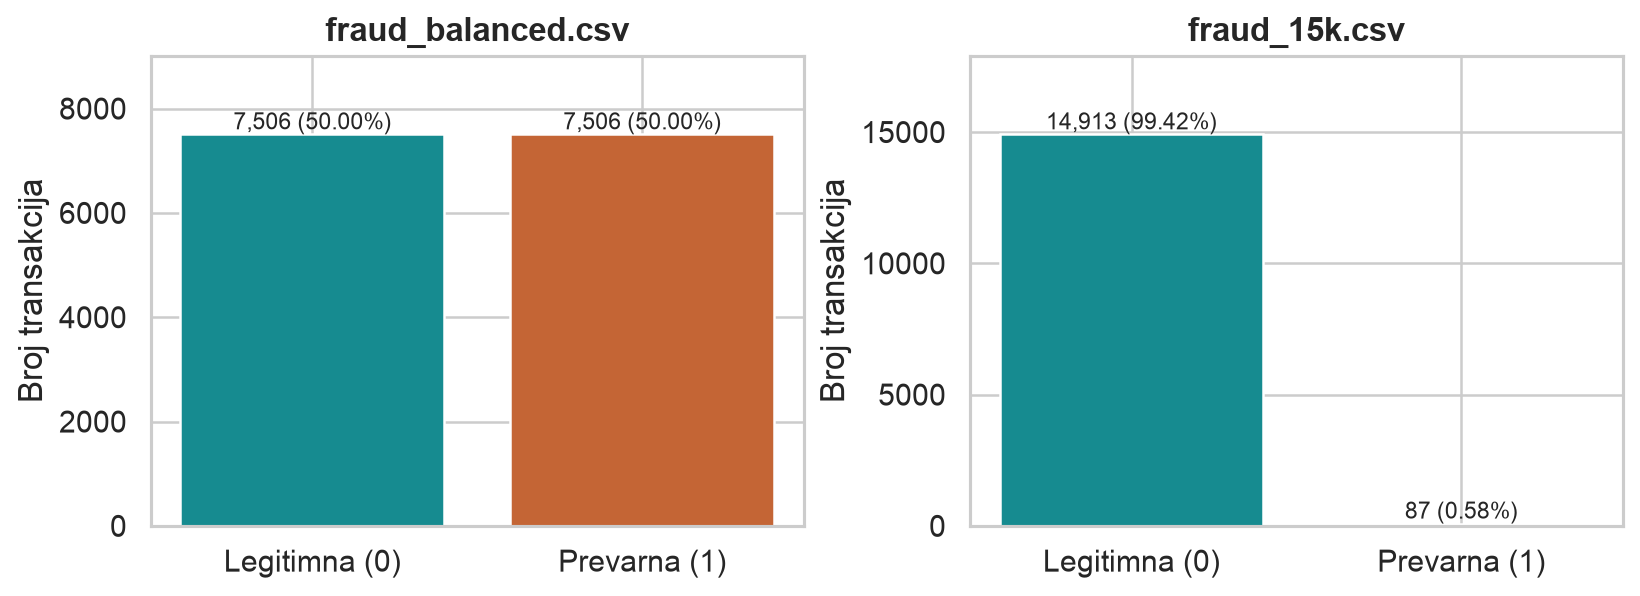
\includegraphics[width=\linewidth,height=.29\textheight,keepaspectratio]{slike/raspodjela_klasa.png}
\caption{Broj i udio klasa u dva ulazna CSV-a. Balansirani odnos formira se nasumičnim smanjivanjem većinske klase.}
\end{figure}

\subsubsection*{Zbirni pregled svih izvornih atributa}
Tabela sažima opis svih varijabli. U njoj su obuhvaćene i kolone koje će se
kasnije izostaviti iz ulaza. Izostavljanje iz pripreme ne zamjenjuje analizu:
odluka se zasniva na značenju, kvalitetu i zastupljenosti vrijednosti. Rasponi su prikazani u izvornim jedinicama, a potpune frekvencije
ostaju dostupne u bilježnici.
\begingroup\small\setlength{\tabcolsep}{3pt}
\begin{longtable}{@{}>{\raggedright\arraybackslash}p{.19\linewidth}>{\raggedright\arraybackslash}p{.13\linewidth}>{\raggedright\arraybackslash}p{.28\linewidth}>{\raggedright\arraybackslash}p{.34\linewidth}@{}}
\caption{Pojedinačni pregled svih 22 atributa balansiranog skupa}\label{tab:eda_atributi}\\
\toprule Atribut & Tip & Raspon / sažetak & Zapažanje \\ \midrule\endfirsthead
\toprule Atribut & Tip & Raspon / sažetak & Zapažanje \\ \midrule\endhead
\bottomrule\endfoot
\texttt{trans\_date\_}\newline\texttt{trans\_time} & datum & 01.01.2019.--21.06.2020. & Nepotpun posljednji mjesec; izražena koncentracija prevara u noćnim satima. \\
\texttt{cc\_num} & oznaka & 977 vrijednosti; najčešća 630451534402 (38) & Ista kartica se ponavlja kroz različite transakcije. \\
\texttt{merchant} & kategorički & 693 vrijednosti; najčešća fraud\_Kilback LLC (72) & Zajednički prefiks fraud\_ ne razlikuje klase; mnogo rijetkih trgovaca. \\
\texttt{category} & kategorički & 14 vrijednosti; najčešća grocery\_pos (2494) & 14 vrsta kupovine; različita zastupljenost po klasi. \\
\texttt{amt} & numerički & 1,00 do 6\,337,25 & Desna asimetrija 1,48; najveći iznos pripada legitimnoj transakciji. \\
\texttt{first} & kategorički & 352 vrijednosti; najčešća Christopher (330) & Ime se ponavlja i nije jedinstvena oznaka osobe. \\
\texttt{last} & kategorički & 480 vrijednosti; najčešća Smith (301) & Prezime se ponavlja kroz transakcije i korisnike. \\
\texttt{gender} & kategorički & 2 vrijednosti; najčešća F (7835) & Dvije nominalne kategorije; bez poretka. \\
\texttt{street} & kategorički & 977 vrijednosti; najčešća 561 Little Plain Apt. 738 (38) & Adresa se ponavlja u kupovinama iste kartice. \\
\texttt{city} & kategorički & 889 vrijednosti; najčešća Warren (57) & Mnogo različitih oznaka; naziv grada nije jednoznačan bez države. \\
\texttt{state} & kategorički & 51 vrijednosti; najčešća TX (1024) & 51 nominalna oznaka različite zastupljenosti. \\
\texttt{zip} & oznaka & 964 vrijednosti; najčešća 82514 (45) & 964 oznake; 919 četverocifrenih zapisa; broj nije udaljenost. \\
\texttt{lat} & numerički & 20,03 do 66,69 & Dopušten raspon; snažno prati širinu trgovca. \\
\texttt{long} & numerički & -165,67 do -67,95 & Lijeva asimetrija odražava lokacije; vrijednosti su dopuštene. \\
\texttt{city\_pop} & numerički & 23,00 do 2\,906\,700,00 & Izražen desni rep; veliki gradovi ostaju sačuvani. \\
\texttt{job} & kategorički & 493 vrijednosti; najčešća Materials engineer (114) & Mnogo rijetkih zanimanja; broj transakcija nije broj osoba. \\
\texttt{dob} & datum & 30.10.1924.--29.01.2005. & Sva rođenja prethode odgovarajućoj transakciji. \\
\texttt{trans\_num} & oznaka & 15\,012 jedinstvenih oznaka & Sve oznake jedinstvene; provjera duplikata i podjele. \\
\texttt{unix\_time} & numerički & 1\,325\,401\,915,00 do 1\,371\,813\,091,00 & Standardno tumačenje daje godine 2012--2013 umjesto 2019--2020. \\
\texttt{merch\_lat} & numerički & 19,04 do 67,51 & Jaka povezanost sa geografskom širinom korisnika. \\
\texttt{merch\_long} & numerički & -166,55 do -67,03 & Jaka povezanost sa geografskom dužinom korisnika. \\
\texttt{is\_fraud} & cilj & 2 vrijednosti; najčešća 1 (7506) & Cilj 0/1; po 7.506 redova, odvojen od ulaza. \\
\end{longtable}\endgroup



\subsubsection*{Kako čitamo numeričke raspodjele}
Aritmetička sredina opisuje prosječnu vrijednost, ali je osjetljiva na velike
vrijednosti u repu. Medijan dijeli posmatranja na dvije jednake polovine, a kvartili
ograničavaju središnjih 50\,\% podataka. Standardna devijacija opisuje rasipanje
oko sredine. Zajedno daju više informacija nego pojedinačan pokazatelj, posebno
za iznos i veličinu grada kod kojih se sredina i medijan znatno razlikuju.

Koeficijent asimetrije opisuje smjer i izraženost repa. Vrijednosti između
$-0{,}5$ i $0{,}5$ ovdje označavaju približnu simetriju, apsolutne vrijednosti
između $0{,}5$ i $1$ umjerenu asimetriju, a veće od $1$ jaku asimetriju.
Ova podjela služi opisu asimetrije, a ne kao test kojim se svaka raspodjela
mora pretvoriti u normalnu. Približna simetrija također ne dokazuje normalnost raspodjele.

Box plot prikazuje medijan, kvartile i statistički izdvojene vrijednosti.
Za $IQR=Q_3-Q_1$ koristimo granice $Q_1-1{,}5IQR$ i $Q_3+1{,}5IQR$.
Tačke izvan njih posmatraju se dodatno. Kod geografske širine ili populacije grada
one mogu jednostavno predstavljati rjeđe lokacije. Zato IQR nije upotrijebljen kao
automatsko pravilo za izbacivanje transakcija.

Histogram prikazuje koncentraciju vrijednosti po intervalima, dok KDE predstavlja
izglađenu procjenu gustoće. Oblik KDE zavisi i od izglađivanja, pa male talase ne
tumačimo kao dokaz zasebnih grupa. Za diskretne veličine, poput sata, frekvencije
su neposredniji prikaz, a KDE je dopunski. Logaritamska osa samo mijenja prikaz
izvornih vrijednosti; stvarna transformacija \texttt{log1p} provjerava se zasebno.
\begin{table}[H]\centering
\caption{Numerička statistika balansiranog skupa; n je broj IQR izdvajanja}\label{tab:numericke}
\small\resizebox{\linewidth}{!}{\begin{tabular}{@{}lrrrrrrr@{}}\toprule
Atribut & Sredina & $s$ & Min. & Medijan & Maks. & Skew & $n$ \\ \midrule
amt & 299,52 & 373,92 & 1,00 & 89,55 & 6\,337,25 & 1,48 & 118 \\
lat & 38,62 & 5,13 & 20,03 & 39,41 & 66,69 & 0,03 & 66 \\
long & -90,28 & 14,08 & -165,67 & -87,41 & -67,95 & -1,20 & 491 \\
city\_pop & 90\,510,75 & 303\,554,43 & 23,00 & 2\,526,00 & 2\,906\,700,00 & 5,62 & 2774 \\
unix\_time ($10^9$ s) & 1,3488 & 0,0133 & 1,3254 & 1,3489 & 1,3718 & 0,00 & 0 \\
merch\_lat & 38,61 & 5,17 & 19,04 & 39,40 & 67,51 & 0,03 & 79 \\
merch\_long & -90,28 & 14,11 & -166,55 & -87,36 & -67,03 & -1,19 & 480 \\
age\_years & 47,57 & 18,06 & 13,99 & 46,05 & 95,48 & 0,48 & 0 \\
distance\_km & 76,38 & 28,85 & 0,74 & 78,39 & 144,52 & -0,24 & 0 \\
hour & 13,30 & 8,37 & 0,00 & 15,00 & 23,00 & -0,30 & 0 \\
day\_of\_week & 3,10 & 2,13 & 0,00 & 3,00 & 6,00 & -0,10 & 0 \\
month & 5,86 & 3,43 & 1,00 & 5,00 & 12,00 & 0,37 & 0 \\
\bottomrule\end{tabular}}
\end{table}


\subsubsection*{Iznos transakcije (\texttt{amt})}

Iznos je pozitivna novčana veličina izražena u USD. Sredina je približno 299,52,
a medijan 89,55 USD. Razlika pokazuje da desni rep znatno utiče na prosjek.
Koeficijent asimetrije od oko 1,48 potvrđuje izraženu asimetriju udesno.
Raspon do 6\,337,25 USD obuhvata i ispravne velike transakcije.

\begin{figure}[H]\centering
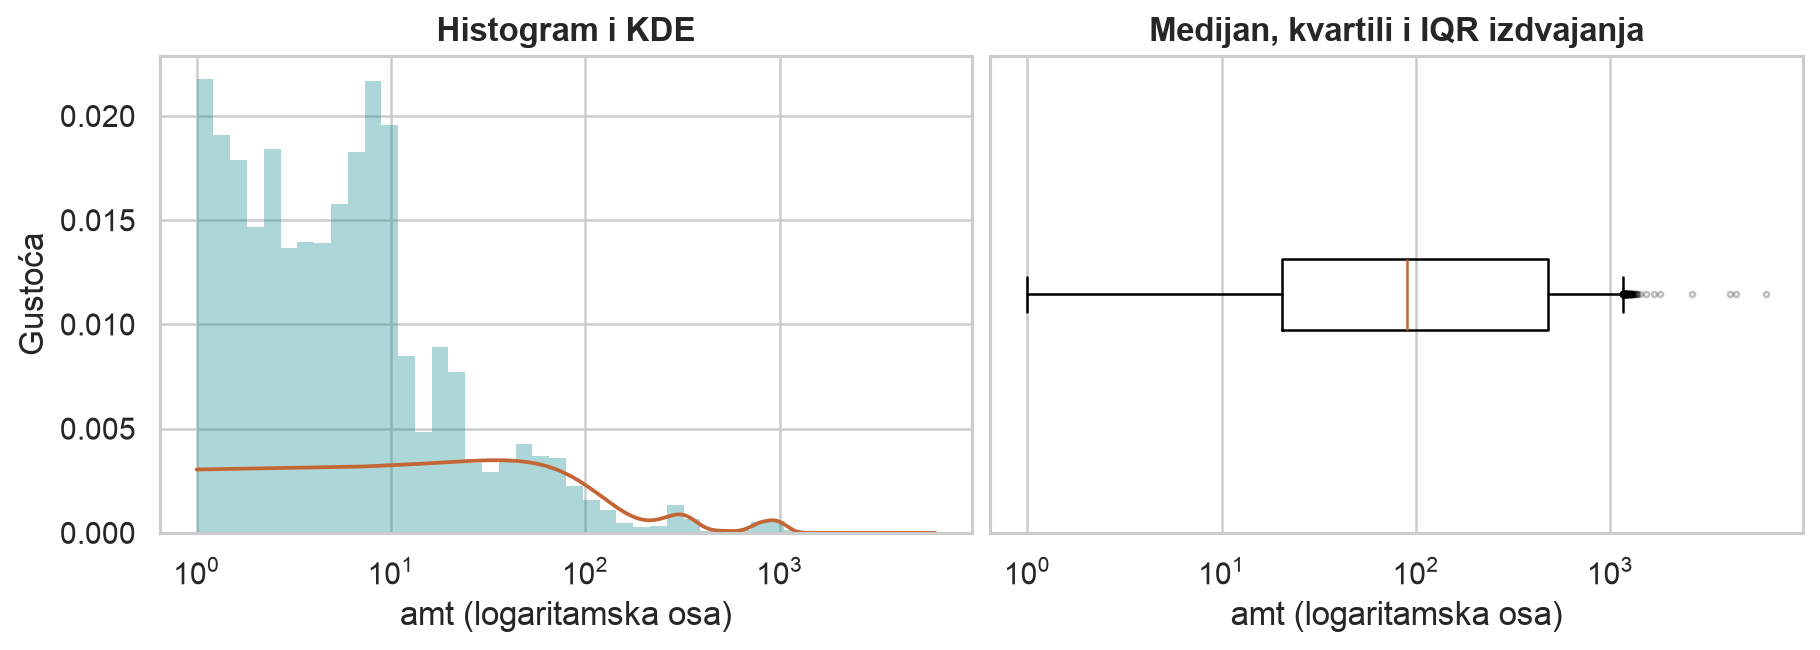
\includegraphics[width=\linewidth,height=.27\textheight,keepaspectratio]{slike/profil_amt.png}
\caption{Pojedinačni profil: amt. Histogram i KDE opisuju oblik raspodjele, a box plot kvartile i izdvojene vrijednosti.}
\end{figure}

\subsubsection*{Geografska širina korisnika (\texttt{lat})}

Širina opisuje lokaciju korisnika u stepenima. Raspon približno 20,03--66,69
nalazi se unutar dozvoljenog geografskog intervala. Sredina i medijan su bliski,
a asimetrija je oko 0,03. Ipak, histogram ima više lokalnih koncentracija jer
transakcije potiču s ponovljenih lokacija, a ne iz ravnomjerno naseljenog prostora.

\begin{figure}[H]\centering
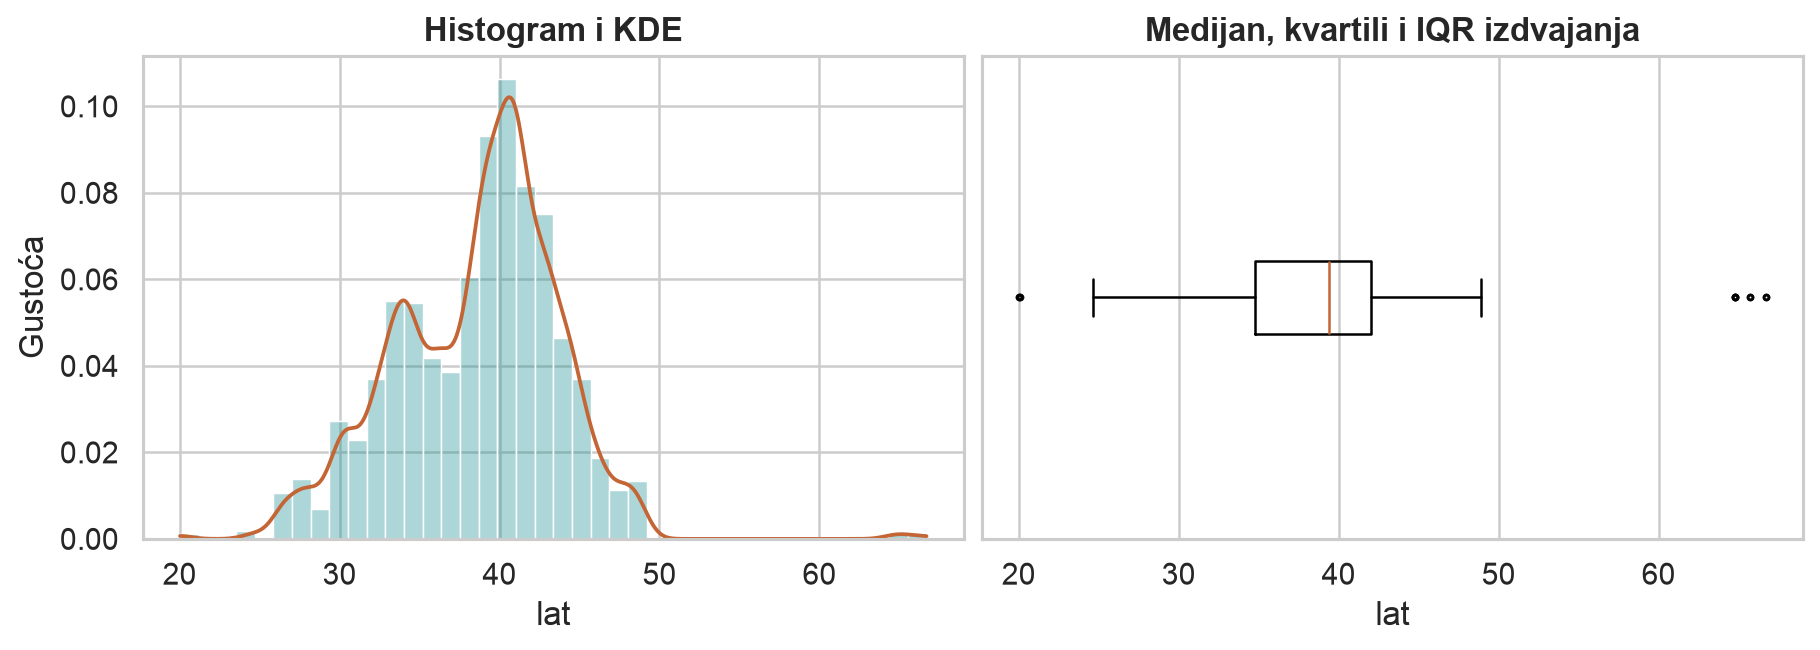
\includegraphics[width=\linewidth,height=.27\textheight,keepaspectratio]{slike/profil_lat.png}
\caption{Pojedinačni profil: lat. Histogram i KDE opisuju oblik raspodjele, a box plot kvartile i izdvojene vrijednosti.}
\end{figure}

\subsubsection*{Geografska dužina korisnika (\texttt{long})}

Dužina sadrži negativne vrijednosti zbog lokacija na zapadnoj hemisferi.
Negativan predznak je dio geografskog značenja i nije greška koju treba ispravljati.
Raspon je približno od $-165{,}67$ do $-67{,}95$ stepeni. Asimetrija oko $-1{,}20$
opisuje duži lijevi rep u rasporedu zastupljenih lokacija.

\begin{figure}[H]\centering
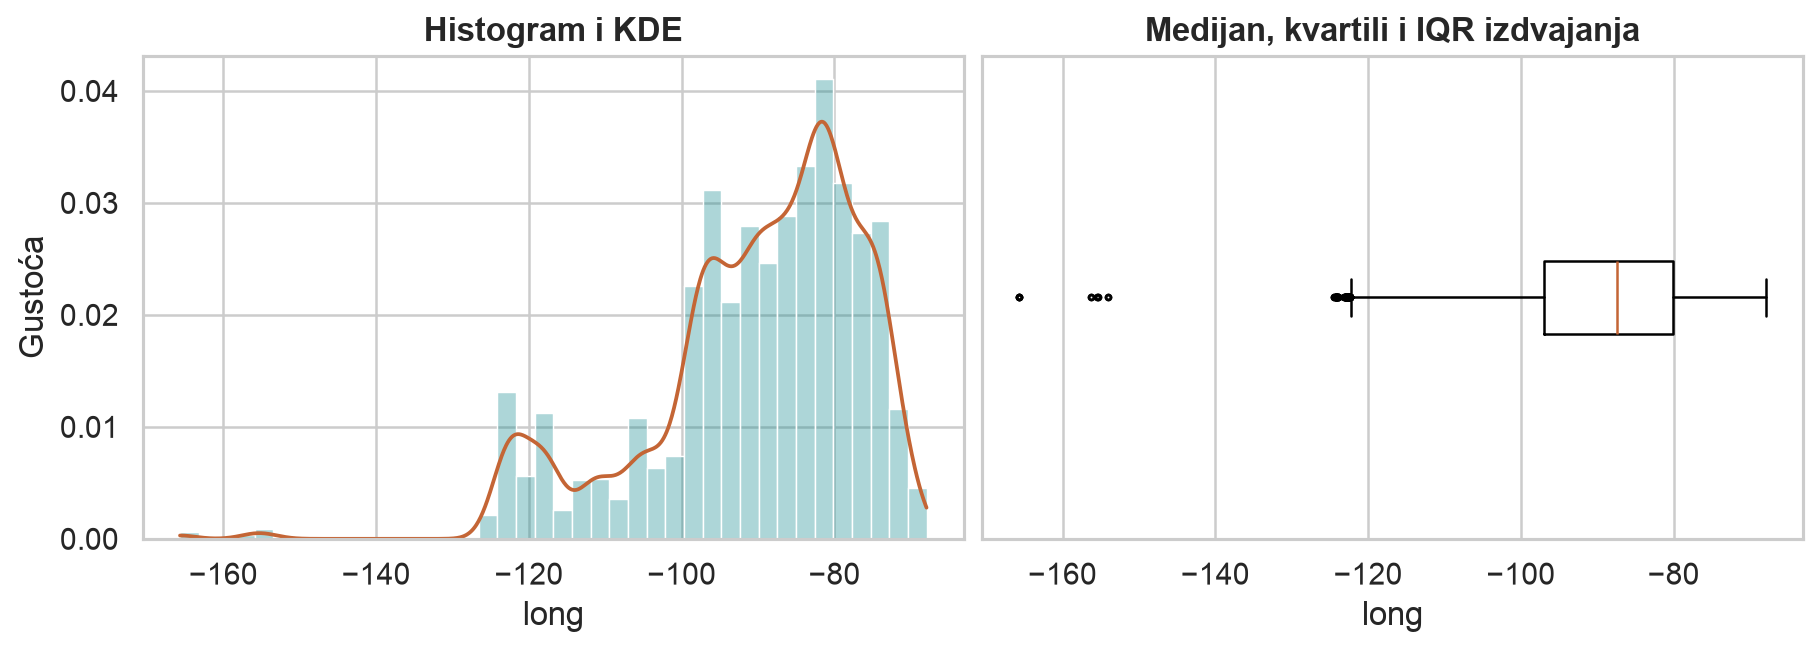
\includegraphics[width=\linewidth,height=.27\textheight,keepaspectratio]{slike/profil_long.png}
\caption{Pojedinačni profil: long. Histogram i KDE opisuju oblik raspodjele, a box plot kvartile i izdvojene vrijednosti.}
\end{figure}

\subsubsection*{Broj stanovnika grada (\texttt{city\_pop})}

Populacija grada je nenegativna brojčana veličina s vrlo dugim desnim repom.
Medijan je 2\,526 stanovnika, dok je sredina oko 90\,510,75. Maksimum iznosi
2\,906\,700. Razlika nije posljedica zaokruživanja: mali broj transakcija iz
velikih gradova znatno podiže aritmetičku sredinu.

\begin{figure}[H]\centering
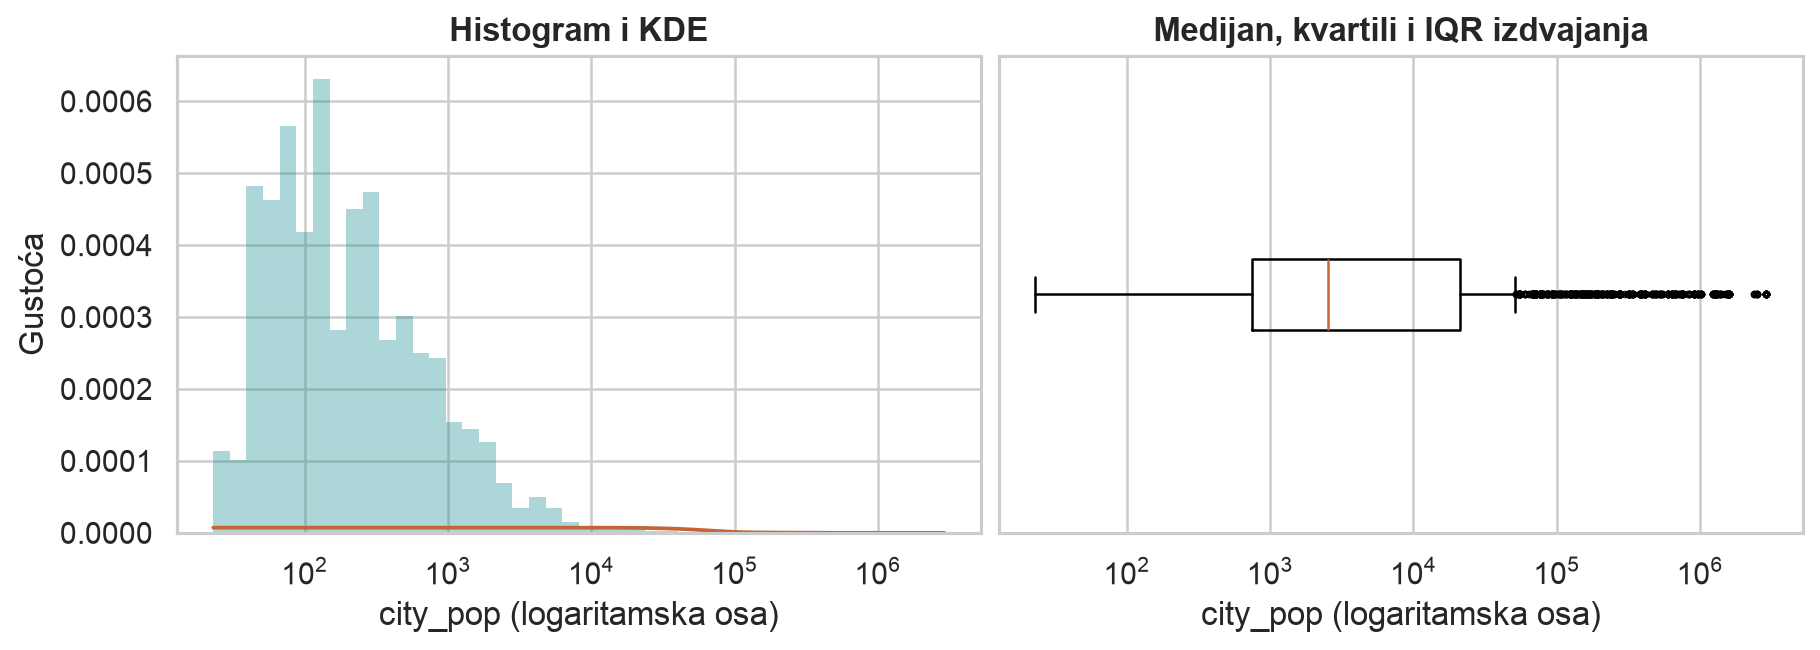
\includegraphics[width=\linewidth,height=.27\textheight,keepaspectratio]{slike/profil_city_pop.png}
\caption{Pojedinačni profil: city\_pop. Histogram i KDE opisuju oblik raspodjele, a box plot kvartile i izdvojene vrijednosti.}
\end{figure}

\subsubsection*{Numerički zapis vremena (\texttt{unix\_time})}

Ova kolona je numerička pohrana vremenske oznake. Zbog potpunosti analize uključena
je u deskriptivnu statistiku, histogram, KDE i box plot, iako neće ostati u konačnim
ulazima. Asimetrija je blizu nule, a IQR ne izdvaja redove. Takav rezultat sam po
sebi ne potvrđuje da je vremenski zapis semantički ispravan.

\begin{figure}[H]\centering
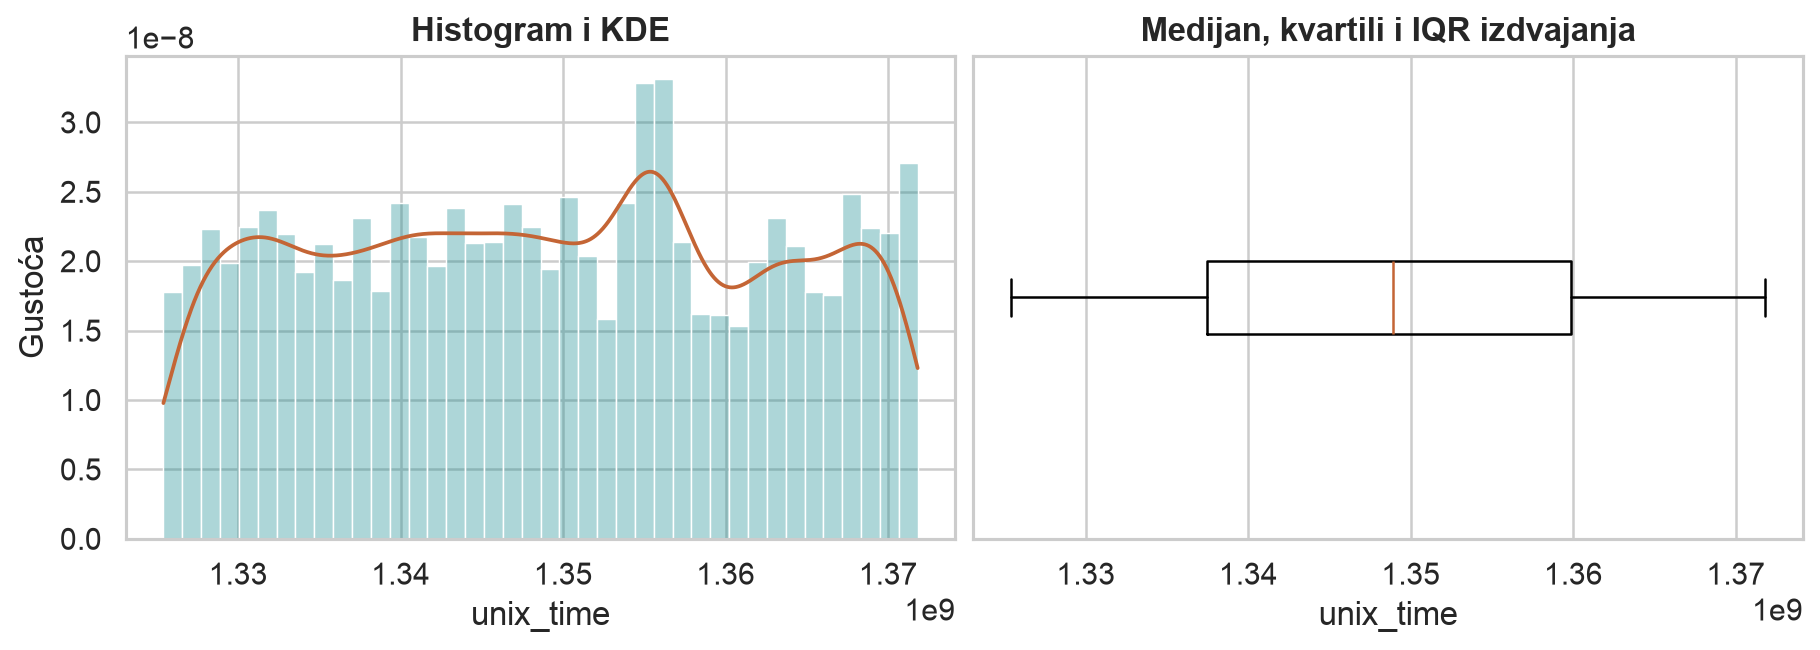
\includegraphics[width=\linewidth,height=.27\textheight,keepaspectratio]{slike/profil_unix_time.png}
\caption{Pojedinačni profil: unix\_time. Histogram i KDE opisuju oblik raspodjele, a box plot kvartile i izdvojene vrijednosti.}
\end{figure}

\subsubsection*{Geografska širina trgovca (\texttt{merch\_lat})}

Širina trgovca ima raspodjelu vrlo sličnu širini korisnika. Sredina je približno
38,61 stepen, a asimetrija oko 0,03. Svi zapisi su unutar dopuštene geografske
širine. IQR izdvaja 79 redova, ali ne ukazuje samostalno na pogrešno unesene
lokacije. Broj izdvajanja zato se navodi kao opis raspodjele.

\begin{figure}[H]\centering
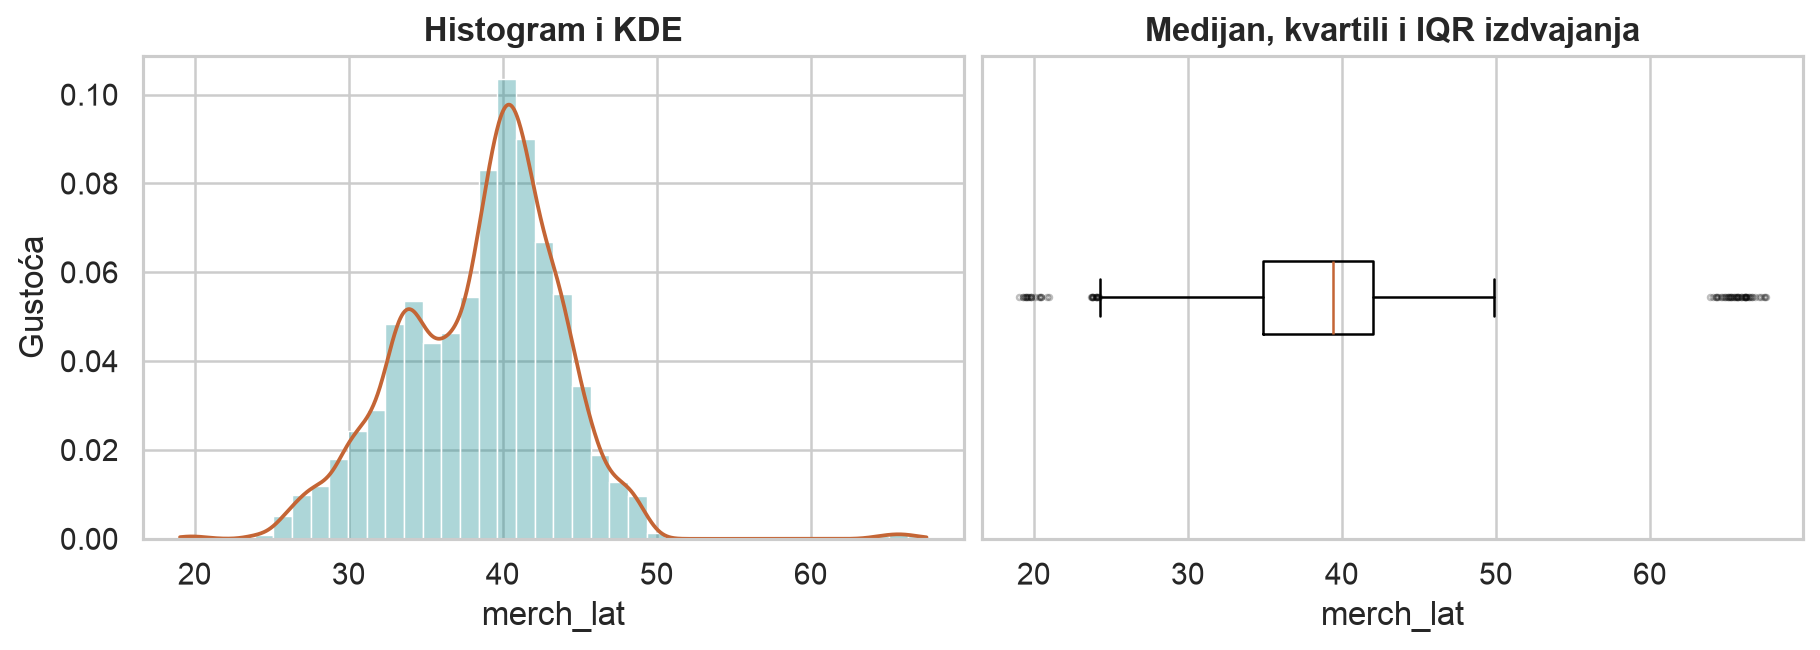
\includegraphics[width=\linewidth,height=.27\textheight,keepaspectratio]{slike/profil_merch_lat.png}
\caption{Pojedinačni profil: merch\_lat. Histogram i KDE opisuju oblik raspodjele, a box plot kvartile i izdvojene vrijednosti.}
\end{figure}

\subsubsection*{Geografska dužina trgovca (\texttt{merch\_long})}

Dužina trgovca prati dužinu korisnika i ima izražen lijevi rep, s asimetrijom
oko $-1{,}19$. Negativne vrijednosti su dopuštene geografske koordinate.
IQR pravilo izdvaja 480 transakcija. Razlika u broju izdvajanja u odnosu na
dužinu korisnika očekivana je jer dvije lokacije nisu potpuno jednake.

\begin{figure}[H]\centering
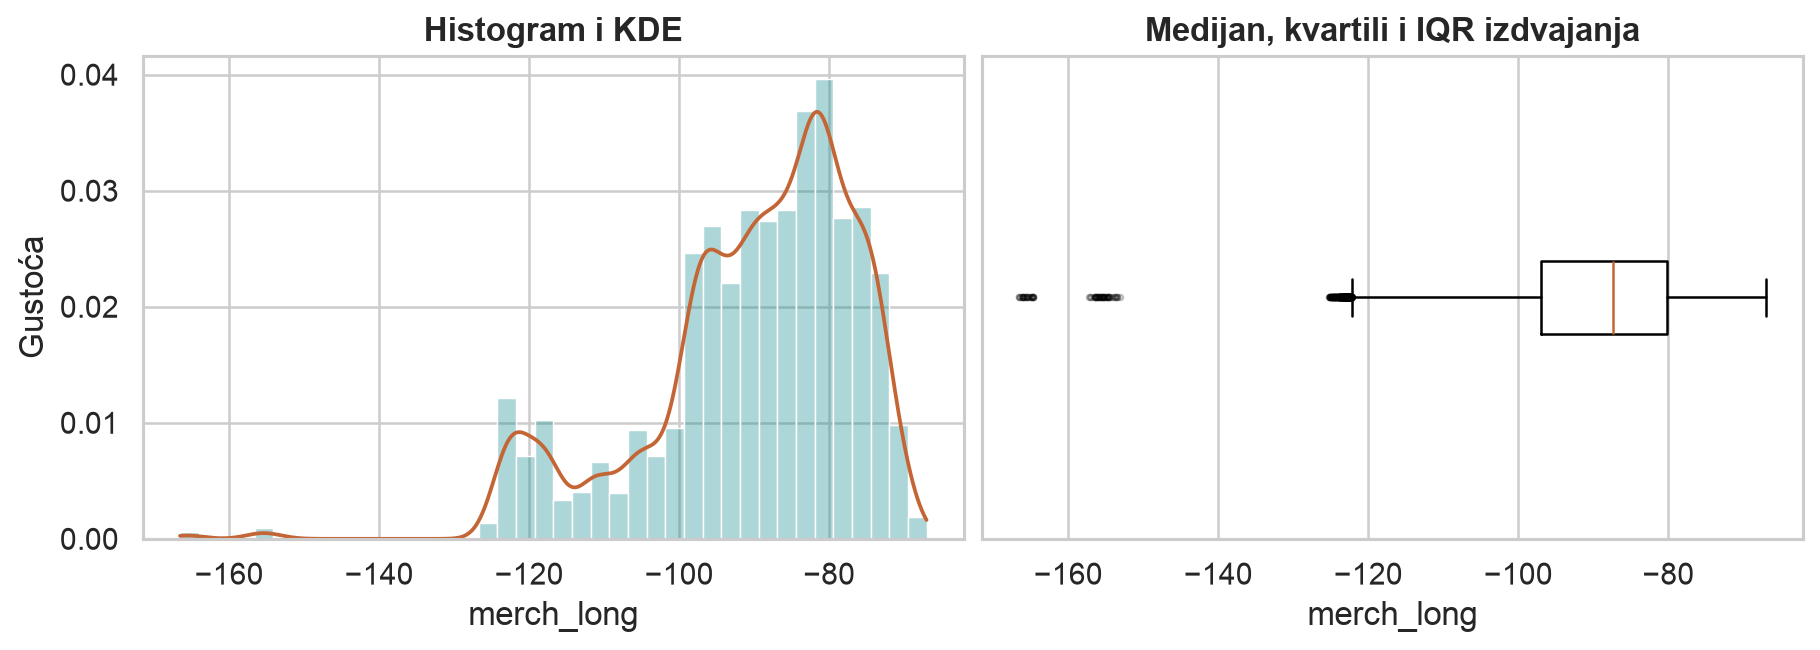
\includegraphics[width=\linewidth,height=.27\textheight,keepaspectratio]{slike/profil_merch_long.png}
\caption{Pojedinačni profil: merch\_long. Histogram i KDE opisuju oblik raspodjele, a box plot kvartile i izdvojene vrijednosti.}
\end{figure}


\subsubsection*{Izdvojene vrijednosti i ciljna klasa}
Zajedničke IQR granice računaju se iz cijelog balansiranog uzorka. Kada se takve
granice primijene posebno na dvije klase, broj izdvojenih redova pokazuje koja
klasa doprinosi repu raspodjele. To nije zamjena za logičku provjeru ispravnosti.
Kod iznosa se posebno vidi da statistički ekstrem može biti legitimna kupovina.


\subsubsection*{Datumi transakcije i datumi rođenja}
Tekstualni datum i vrijeme uspješno se pretvaraju u datumski tip. Najranije i
najkasnije transakcije obuhvataju 1.~1.~2019.--21.~6.~2020. Posljednji mjesec je
nepotpun. Broj transakcija po mjesecu zavisi od dužine posmatranog intervala i
sastava uzorka, pa pad u posljednjem mjesecu ne tumačimo kao samostalnu promjenu
intenziteta kupovine ili učestalosti prevare.

Godina rođenja i datum transakcije omogućavaju određivanje približne starosti u
trenutku događaja. Time se izbjegava računanje starosti prema današnjem datumu,
koje bi promijenilo značenje historijskih transakcija. Koristi se vremenska razlika
u sekundama podijeljena sa 365,2425 dana po godini; vrijednosti se ne zaokružuju prije
dalje obrade. Ovdje se radi o približnoj kontinuiranoj starosti, a ne broju navršenih godina.

Starost se kreće približno od 13,99 do 95,48 godina, sa sredinom 47,57 i medijanom
46,05. U simuliranom skupu nismo našli datum rođenja nakon transakcije. Iz same
starosti ne izvodi se dodatno pravilo za uklanjanje redova. Histogram starosti
ponderisan je brojem transakcija: osoba s većim brojem kupovina pojavljuje se češće.

\begin{figure}[H]\centering
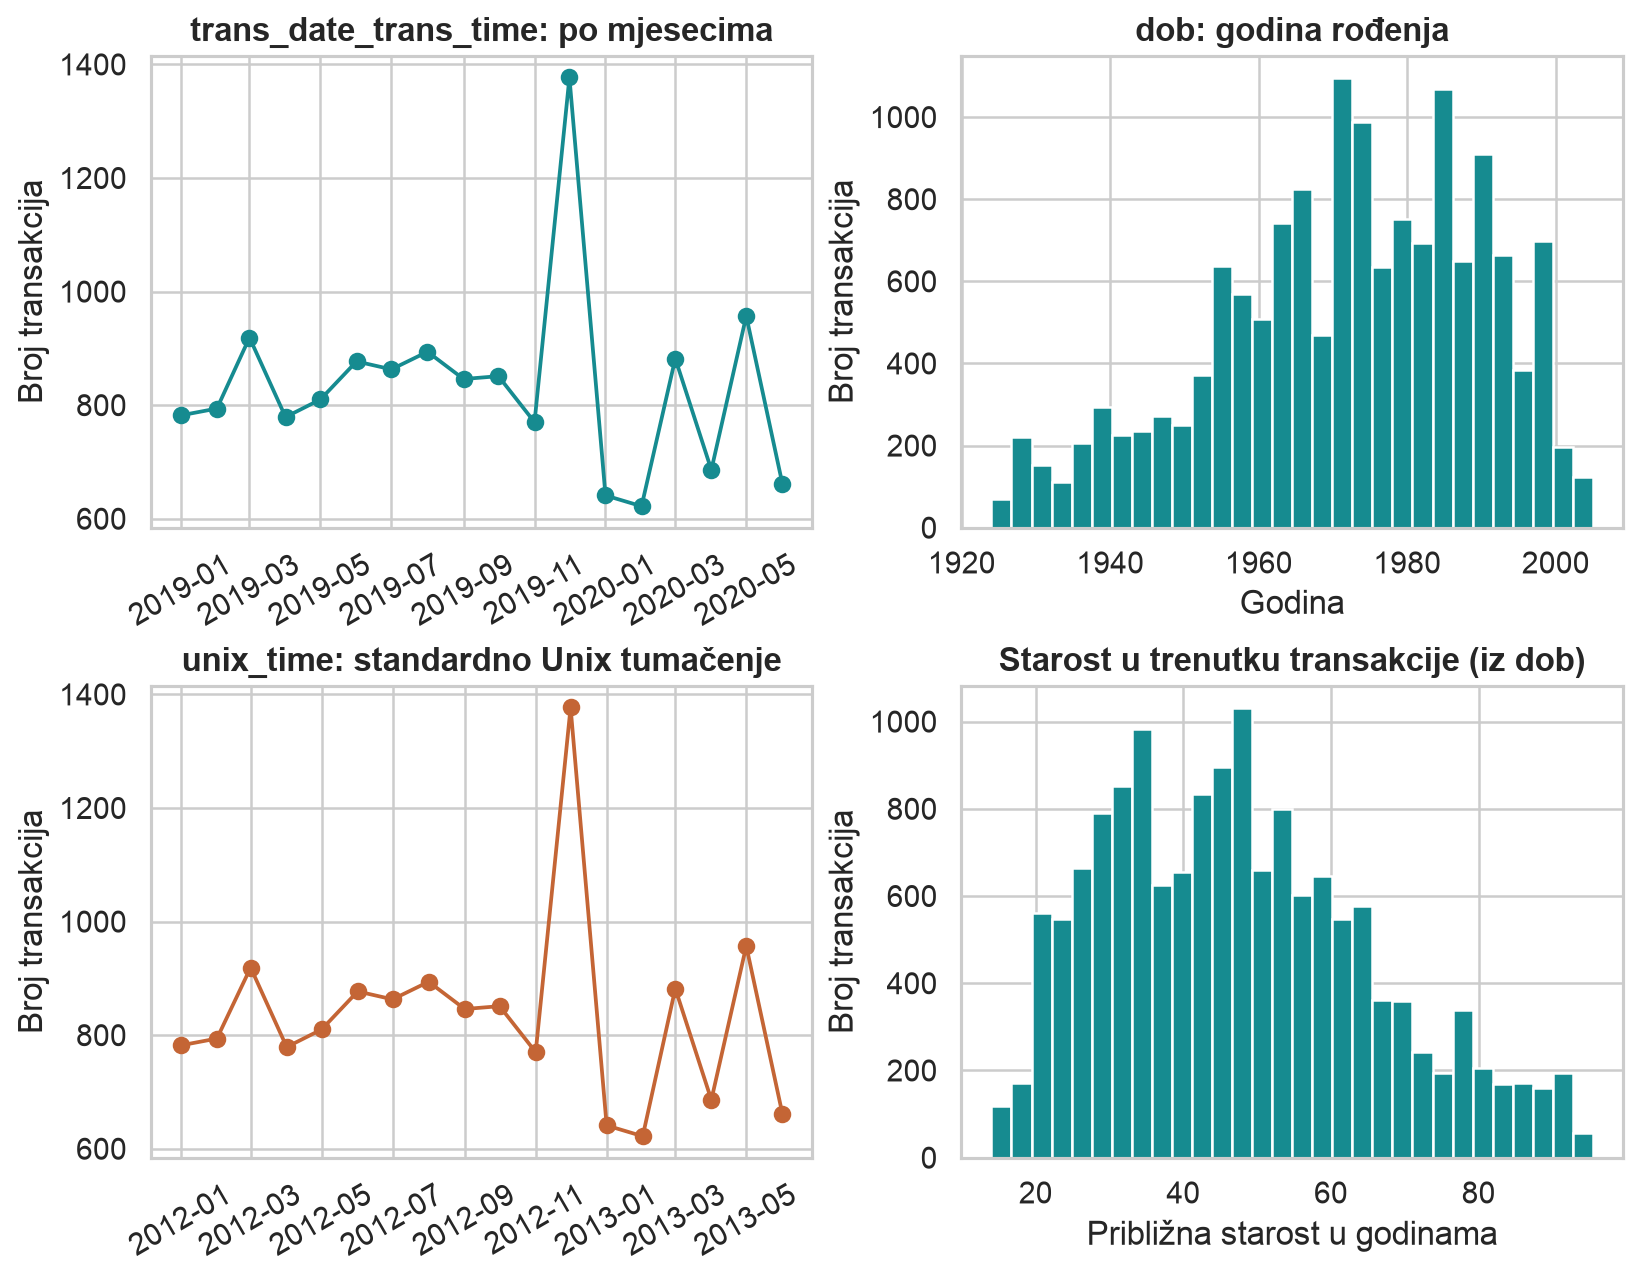
\includegraphics[width=\linewidth,height=.48\textheight,keepaspectratio]{slike/datumi.png}
\caption{Vremenski obuhvat, godine rođenja, neslaganje Unix zapisa i približna starost po transakciji.}
\end{figure}

\subsubsection*{Izvedena starost i udaljenost}
Izvedene veličine analiziraju se jednako kao izvorne: provjeravaju se raspon,
rasipanje, asimetrija i IQR izdvajanja. Izračunavanje nove kolone samo po sebi
ne opravdava njeno zadržavanje. Važno je utvrditi ima li ona razumljivo značenje,
da li uvodi grešku i koju informaciju sažima iz početnog skupa.

Starost ima blagu desnu asimetriju i ne zahtijeva logaritamsku transformaciju.
Udaljenost zračnom linijom ima sredinu približno 76,38 km, medijan 78,39 km i
raspon 0,74--144,52 km u balansiranom uzorku. Njena raspodjela nije izrazito
asimetrična. Sredine po klasama su slične, pa se samoj udaljenosti ne pripisuje
snažno razdvajanje klasa. Njena vrijednost u pripremi je i sažimanje odnosa lokacija.

\begin{figure}[H]\centering
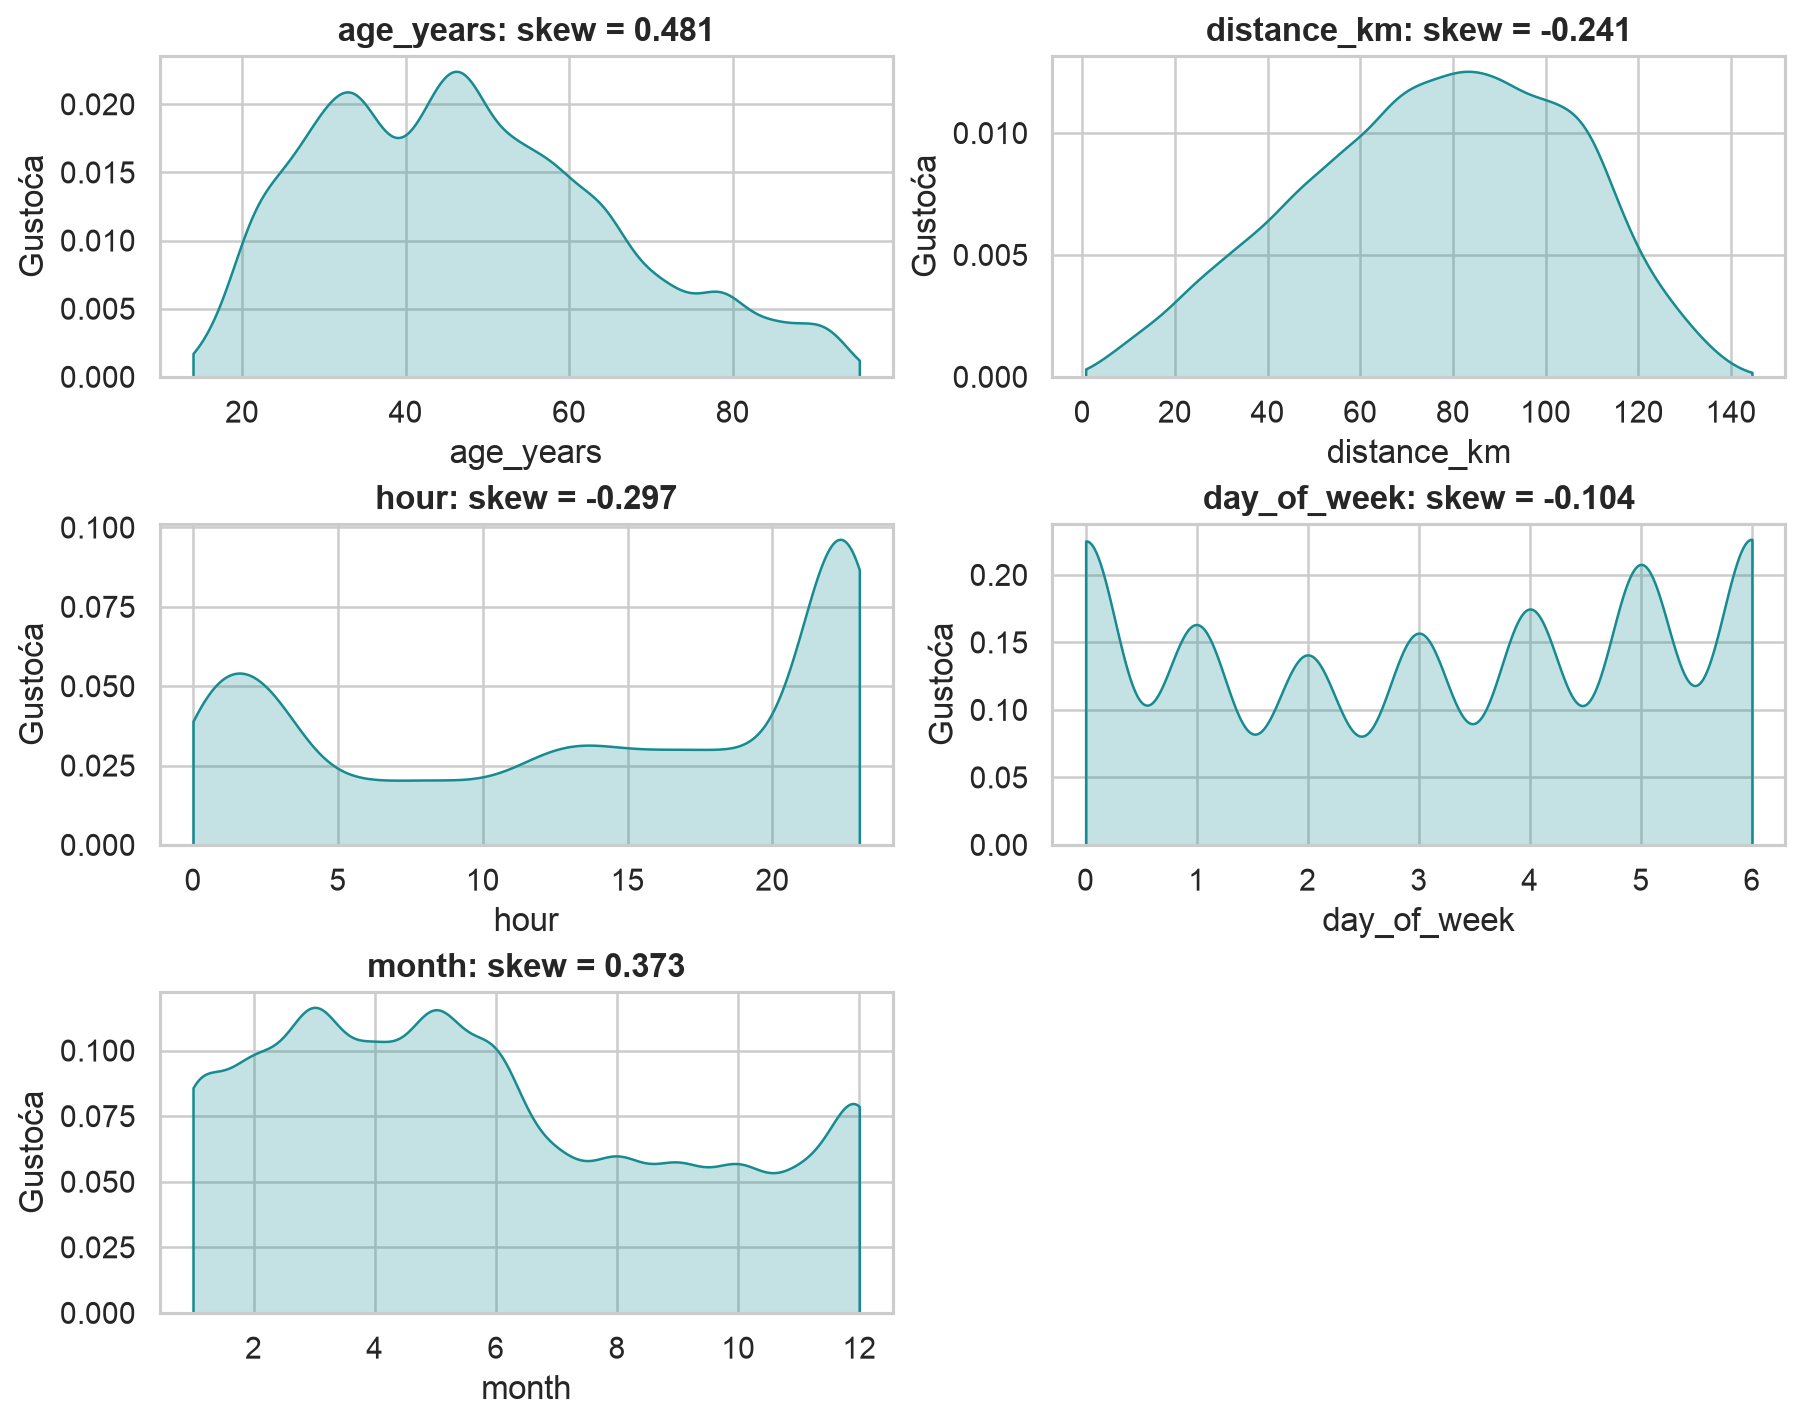
\includegraphics[width=\linewidth,height=.40\textheight,keepaspectratio]{slike/izvedene_gustoce.png}
\caption{Gustoće svih izvedenih veličina. Sat, dan i mjesec su diskretne veličine; KDE je pomoćni prikaz.}
\end{figure}

\begin{figure}[H]\centering
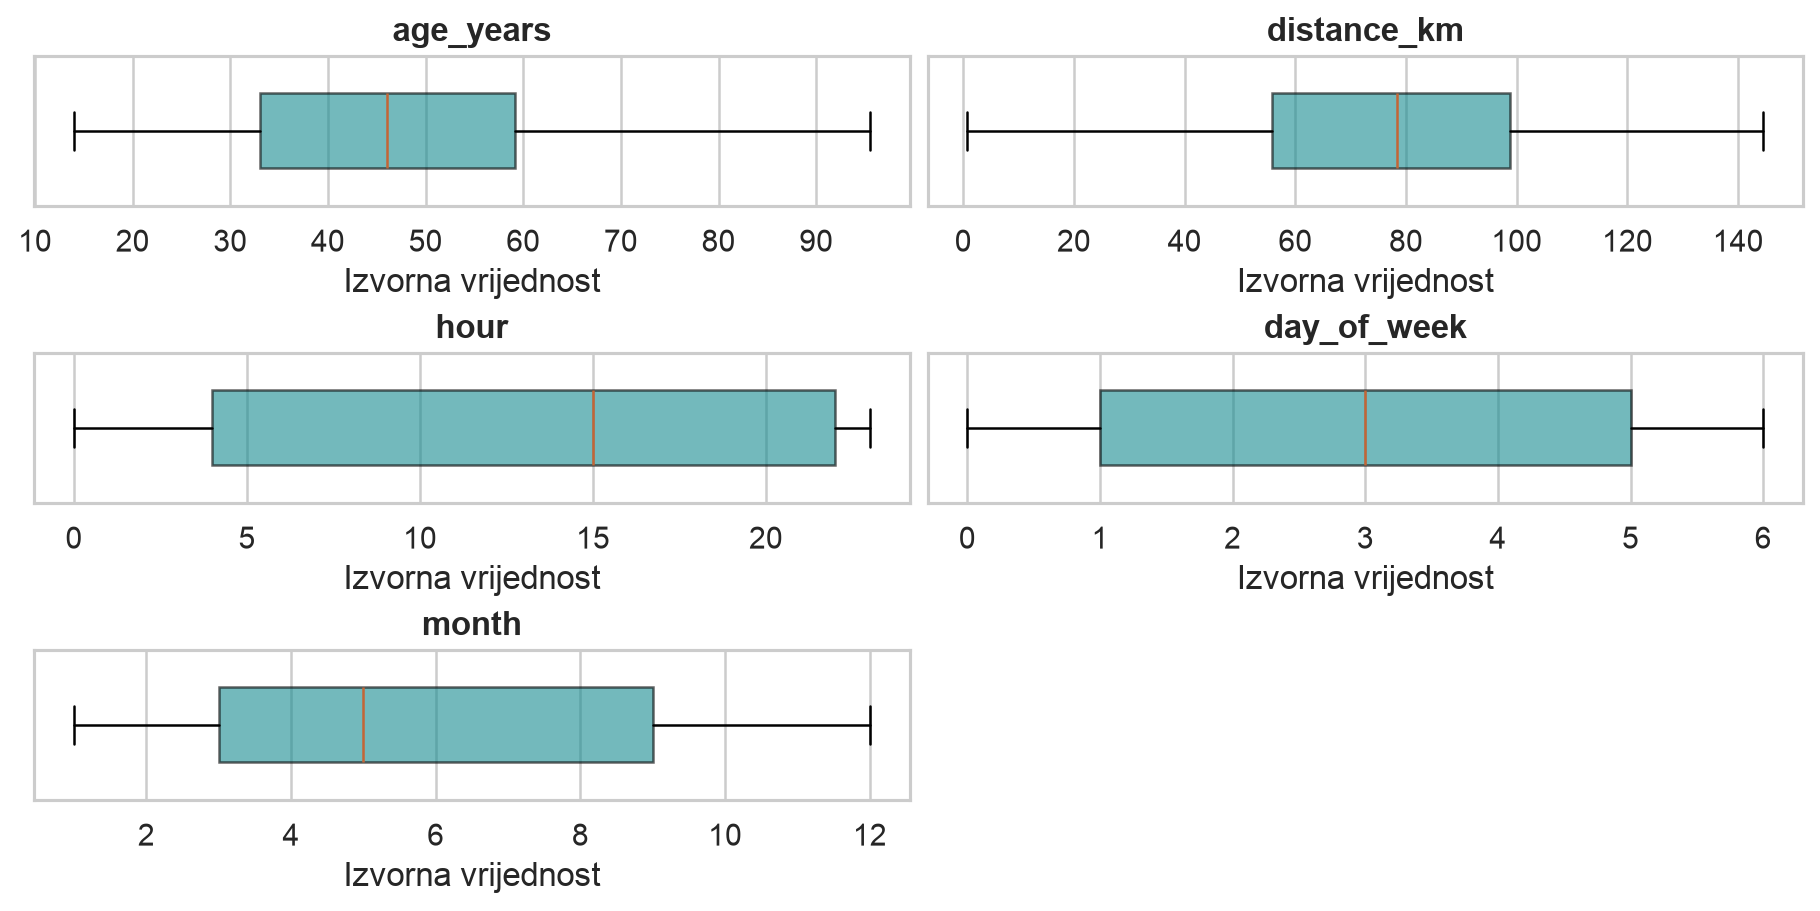
\includegraphics[width=\linewidth,height=.25\textheight,keepaspectratio]{slike/izvedeni_boxplotovi.png}
\caption{Kutijasti prikazi izvedenih veličina; iste granice opisa primjenjuju se prije odluke o transformacijama.}
\end{figure}


\subsubsection*{Sat i dan u sedmici: cikličnost i obrasci klasa}
Sat (0--23) i dan u sedmici (0--6) su ciklični: 23 i 0 su vremenski susjedni,
iako im je brojčana razlika velika. Zato u pripremi čuvamo njihov kružni odnos.

Između 22:00 i 03:59 dešava se 84,76\,\% prevara i 21,72\,\% legitimnih
transakcija u balansiranom uzorku. To su udjeli unutar klase, a ne procjena
rizika noćne kupovine; razlike po danima su manje izražene.

Mala ukupna asimetrija sata ne poništava noćni obrazac. Ista vrijednost asimetrije
može nastati za različite rasporede vrhova, a kružna priroda sata nije sadržana u
tom jednom koeficijentu. Za pripremu zato uvodimo sinus i kosinus sata i dana,
uz periode 24 i 7. Mjesec ostaje u analizi zbog nepotpunog godišnjeg obuhvata.

\begin{figure}[H]\centering
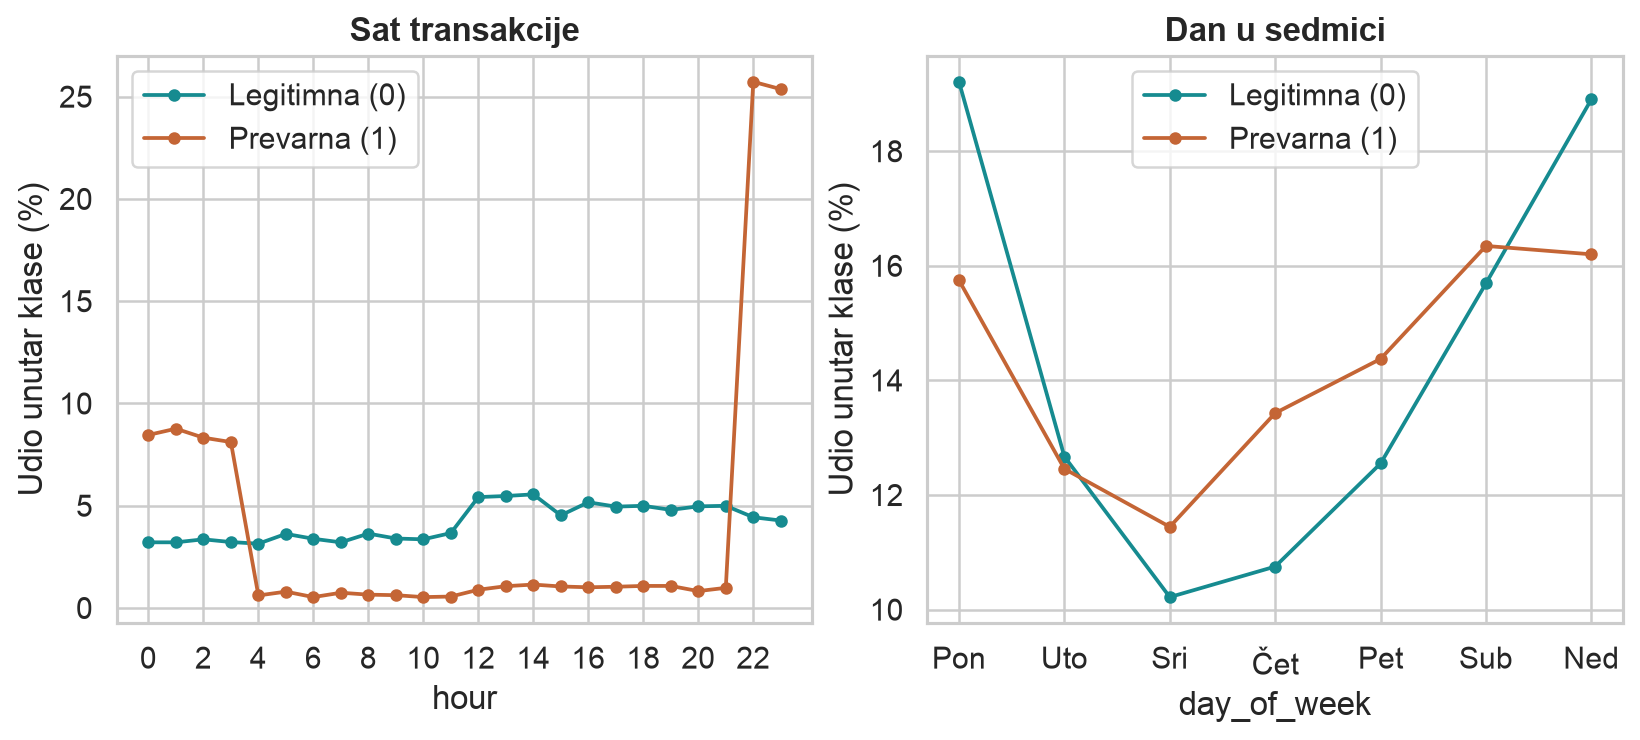
\includegraphics[width=\linewidth,height=.34\textheight,keepaspectratio]{slike/vremenski_obrasci.png}
\caption{Sat i dan u sedmici: udjeli su normalizovani posebno unutar legitimnih i prevarnih transakcija.}
\end{figure}

\subsubsection*{Razlike u iznosima između klasa}
Prosječni iznosi nisu dovoljni da opišu preklapanje klasa. Zato koristimo i
empirijsku kumulativnu raspodjelu te box plot po klasi. Kumulativna kriva na
odabranoj vrijednosti iznosa pokazuje udio transakcija koje imaju taj ili manji iznos.
Na visini 0,5 može se očitati medijan bez pretpostavljanja određenog oblika raspodjele.

Medijan legitimnih iznosa je 47,92 USD, a prevarnih 396,50 USD. Veći iznosi su
zastupljeniji među prevarama u ovom uzorku, ali postoje i male prevare i velike
legitimne kupovine. Najveći iznos, 6\,337,25 USD, pripada legitimnoj transakciji.
Takav nalaz dodatno podržava očuvanje velikih vrijednosti i transformaciju skale
umjesto jednostavnog uklanjanja repa raspodjele.

\begin{figure}[H]\centering
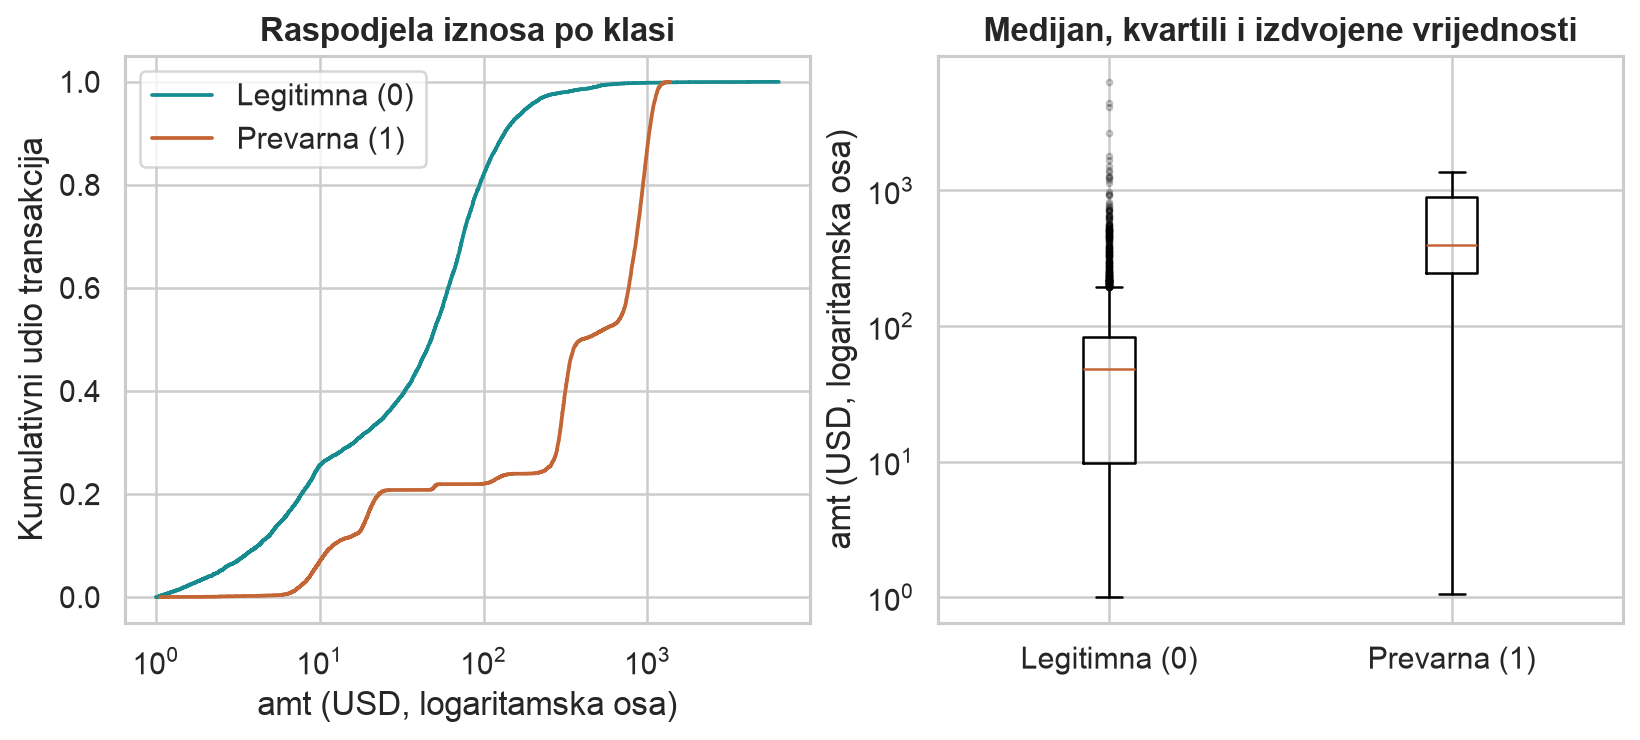
\includegraphics[width=\linewidth,height=.32\textheight,keepaspectratio]{slike/iznos_po_klasi.png}
\caption{Empirijske kumulativne raspodjele i box plot iznosa po klasama; logaritamska osa čuva prikaz cijelog raspona.}
\end{figure}


\subsubsection*{Kategoričke varijable: zastupljenost i rijetke grupe}
Za kategoričke atribute razlikujemo broj različitih oznaka i broj redova koji im
pripada. Veliki broj kategorija može značiti mnogo rijetkih grupa, ali taj odnos
treba izračunati. Zbog toga tabela prikazuje koliko kategorija ima manje od deset
transakcija, koliko ukupno redova one obuhvataju i koliki dio uzorka zauzima deset
najčešćih vrijednosti. Ovi pokazatelji služe opisu, bez korištenja cilja za izbor grupa.

\begin{figure}[H]\centering
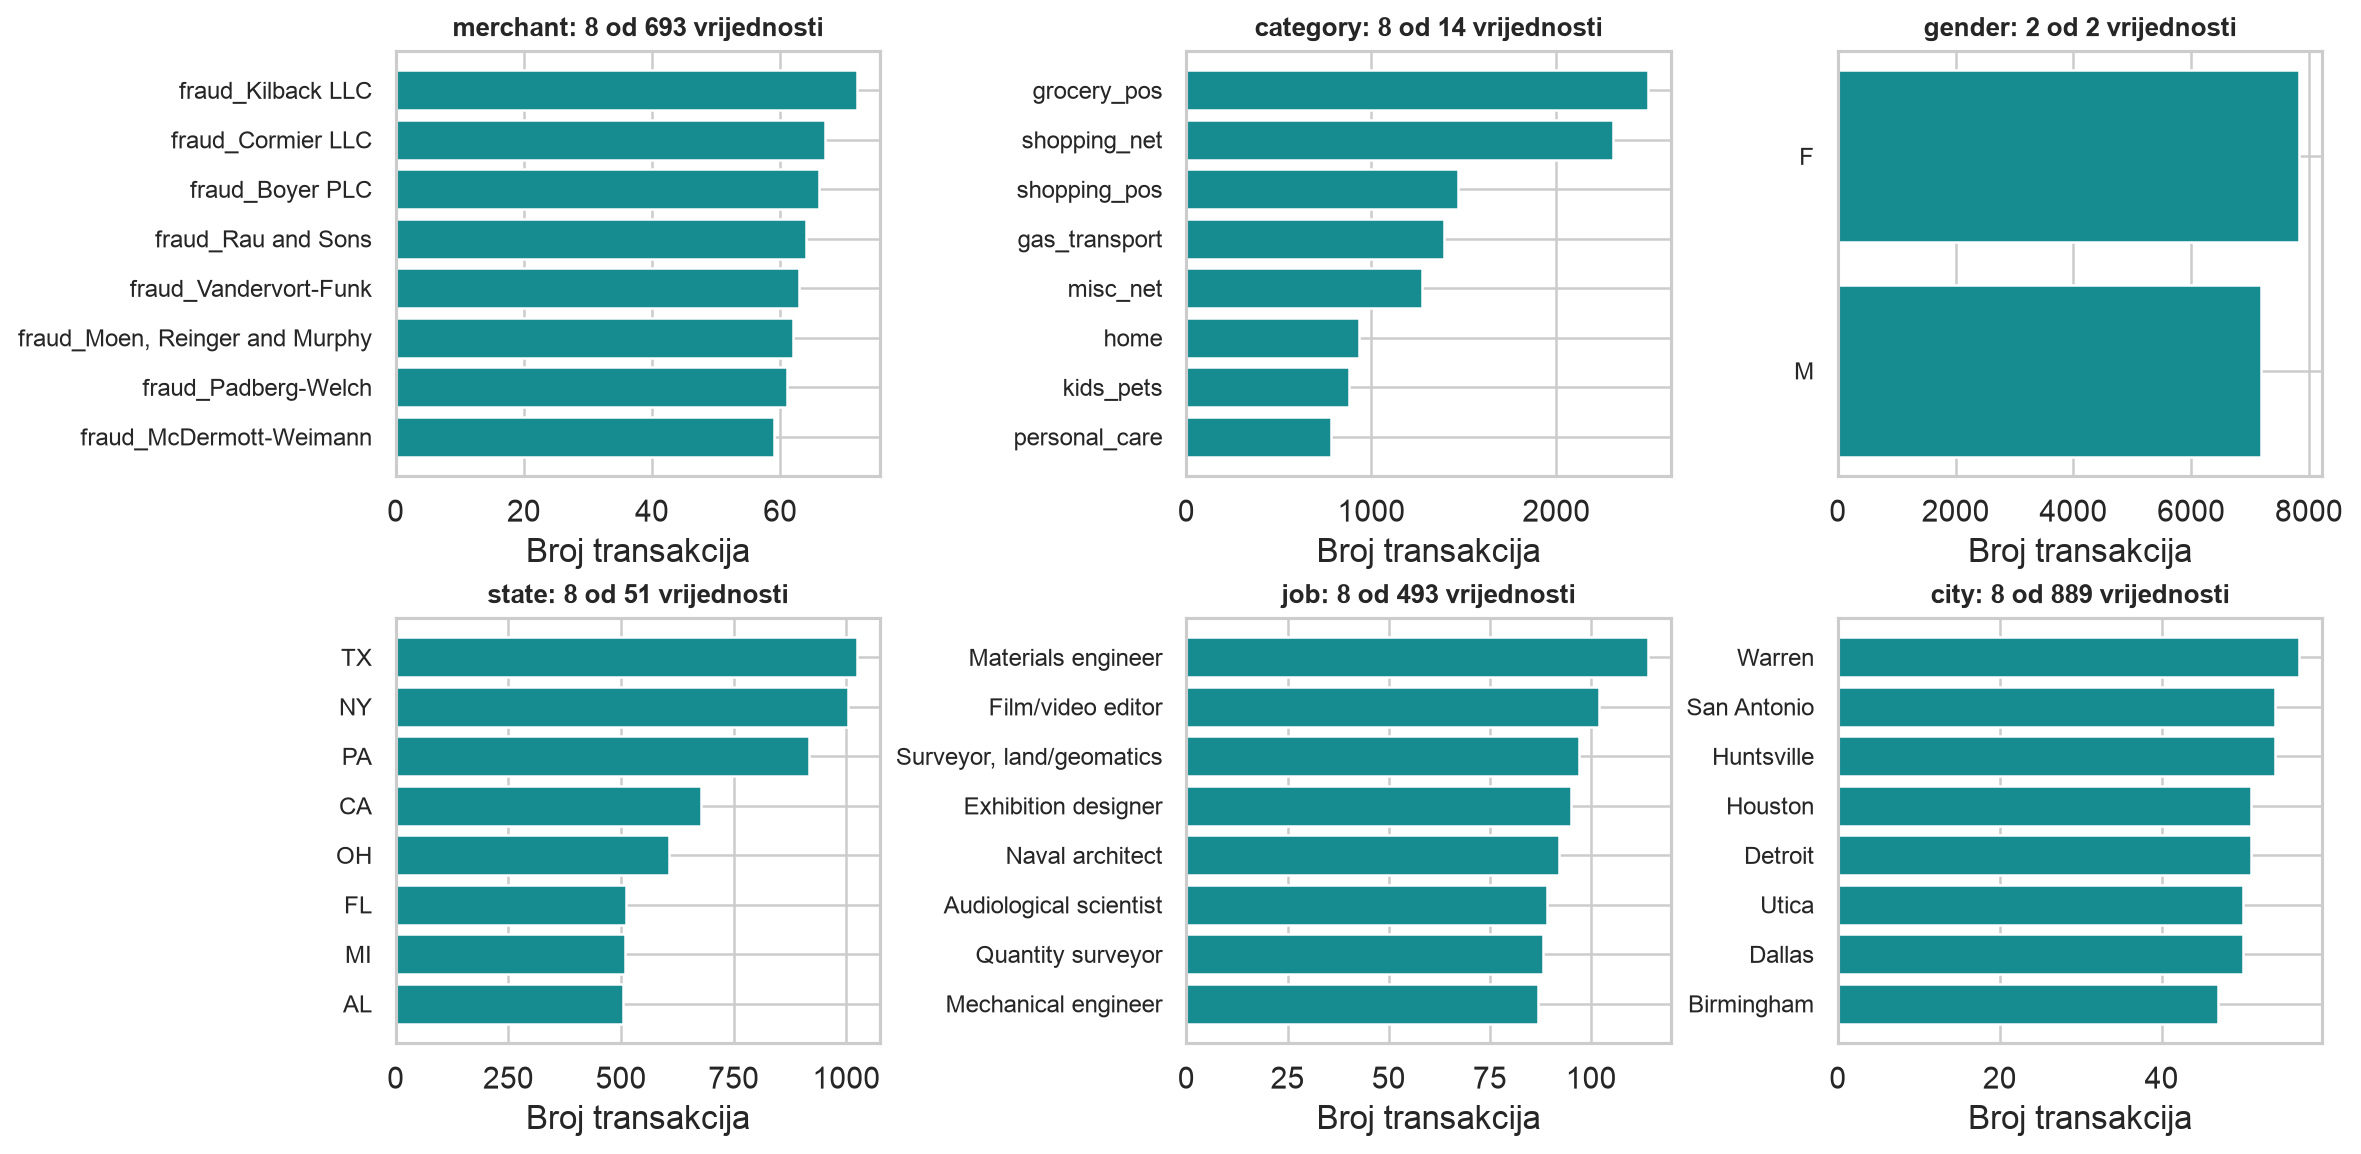
\includegraphics[width=\linewidth,height=.35\textheight,keepaspectratio]{slike/kategoricke_distribucije.png}
\caption{Najčešće vrijednosti šest nominalnih atributa. Prikaz osam vrijednosti nije potpuna raspodjela svih kategorija.}
\end{figure}


\subsubsection*{Vrsta kupovine: svih četrnaest kategorija}
Atribut \texttt{category} opisuje vrstu transakcije i ima 14 vrijednosti.
Kategorije online kupovine i kupovine na prodajnom mjestu predstavljaju različite
vrste događaja, pa se njihove oznake čuvaju odvojeno. Ovaj atribut ima umjeren broj
vrijednosti i jasnije sadržajno značenje od pojedinačnog naziva trgovca.

Najzastupljenija kategorija u balansiranom uzorku je \texttt{grocery\_pos}.
Među svim prevarama posebno su zastupljene \texttt{grocery\_pos} i
\texttt{shopping\_net}. Međutim, kada se gleda udio prevare unutar određene
kategorije, nazivnik je ukupan broj transakcija te kategorije. Zato se tabela
i grafikon čitaju kao odgovori na dva različita pitanja.

Udio prevara po kategoriji prikazan u tabeli uslovljen je odnosom klasa u balansiranom uzorku.
On je koristan za opis uzorka, ali se ne prenosi neposredno kao procjena rizika.
Za pripremu se zadržavaju sve kategorije i kodiraju bez proizvoljnog poretka.
U svakoj od njih ima dovoljno zapisa da se u ovom opisu ne primjenjuje grupisanje
po odabranom pragu za trgovca i zanimanje.
\begin{table}[H]\centering\small
\caption{Struktura svih vrsta kupovine u balansiranom uzorku}
\begin{tabularx}{\linewidth}{@{}Yrrrr@{}}\toprule
Kategorija & Ukupno & Legitimne & Prevare & Udio prevara \\ \midrule
grocery\_pos & 2\,494 & 751 & 1\,743 & 69,89\,\% \\
shopping\_net & 2\,306 & 593 & 1\,713 & 74,28\,\% \\
shopping\_pos & 1\,468 & 625 & 843 & 57,43\,\% \\
gas\_transport & 1\,393 & 775 & 618 & 44,36\,\% \\
misc\_net & 1\,275 & 360 & 915 & 71,76\,\% \\
home & 932 & 734 & 198 & 21,24\,\% \\
kids\_pets & 881 & 642 & 239 & 27,13\,\% \\
personal\_care & 783 & 563 & 220 & 28,10\,\% \\
misc\_pos & 740 & 490 & 250 & 33,78\,\% \\
entertainment & 726 & 493 & 233 & 32,09\,\% \\
food\_dining & 658 & 507 & 151 & 22,95\,\% \\
health\_fitness & 616 & 483 & 133 & 21,59\,\% \\
grocery\_net & 393 & 259 & 134 & 34,10\,\% \\
travel & 347 & 231 & 116 & 33,43\,\% \\
\bottomrule\end{tabularx}\end{table}


\begin{figure}[H]\centering
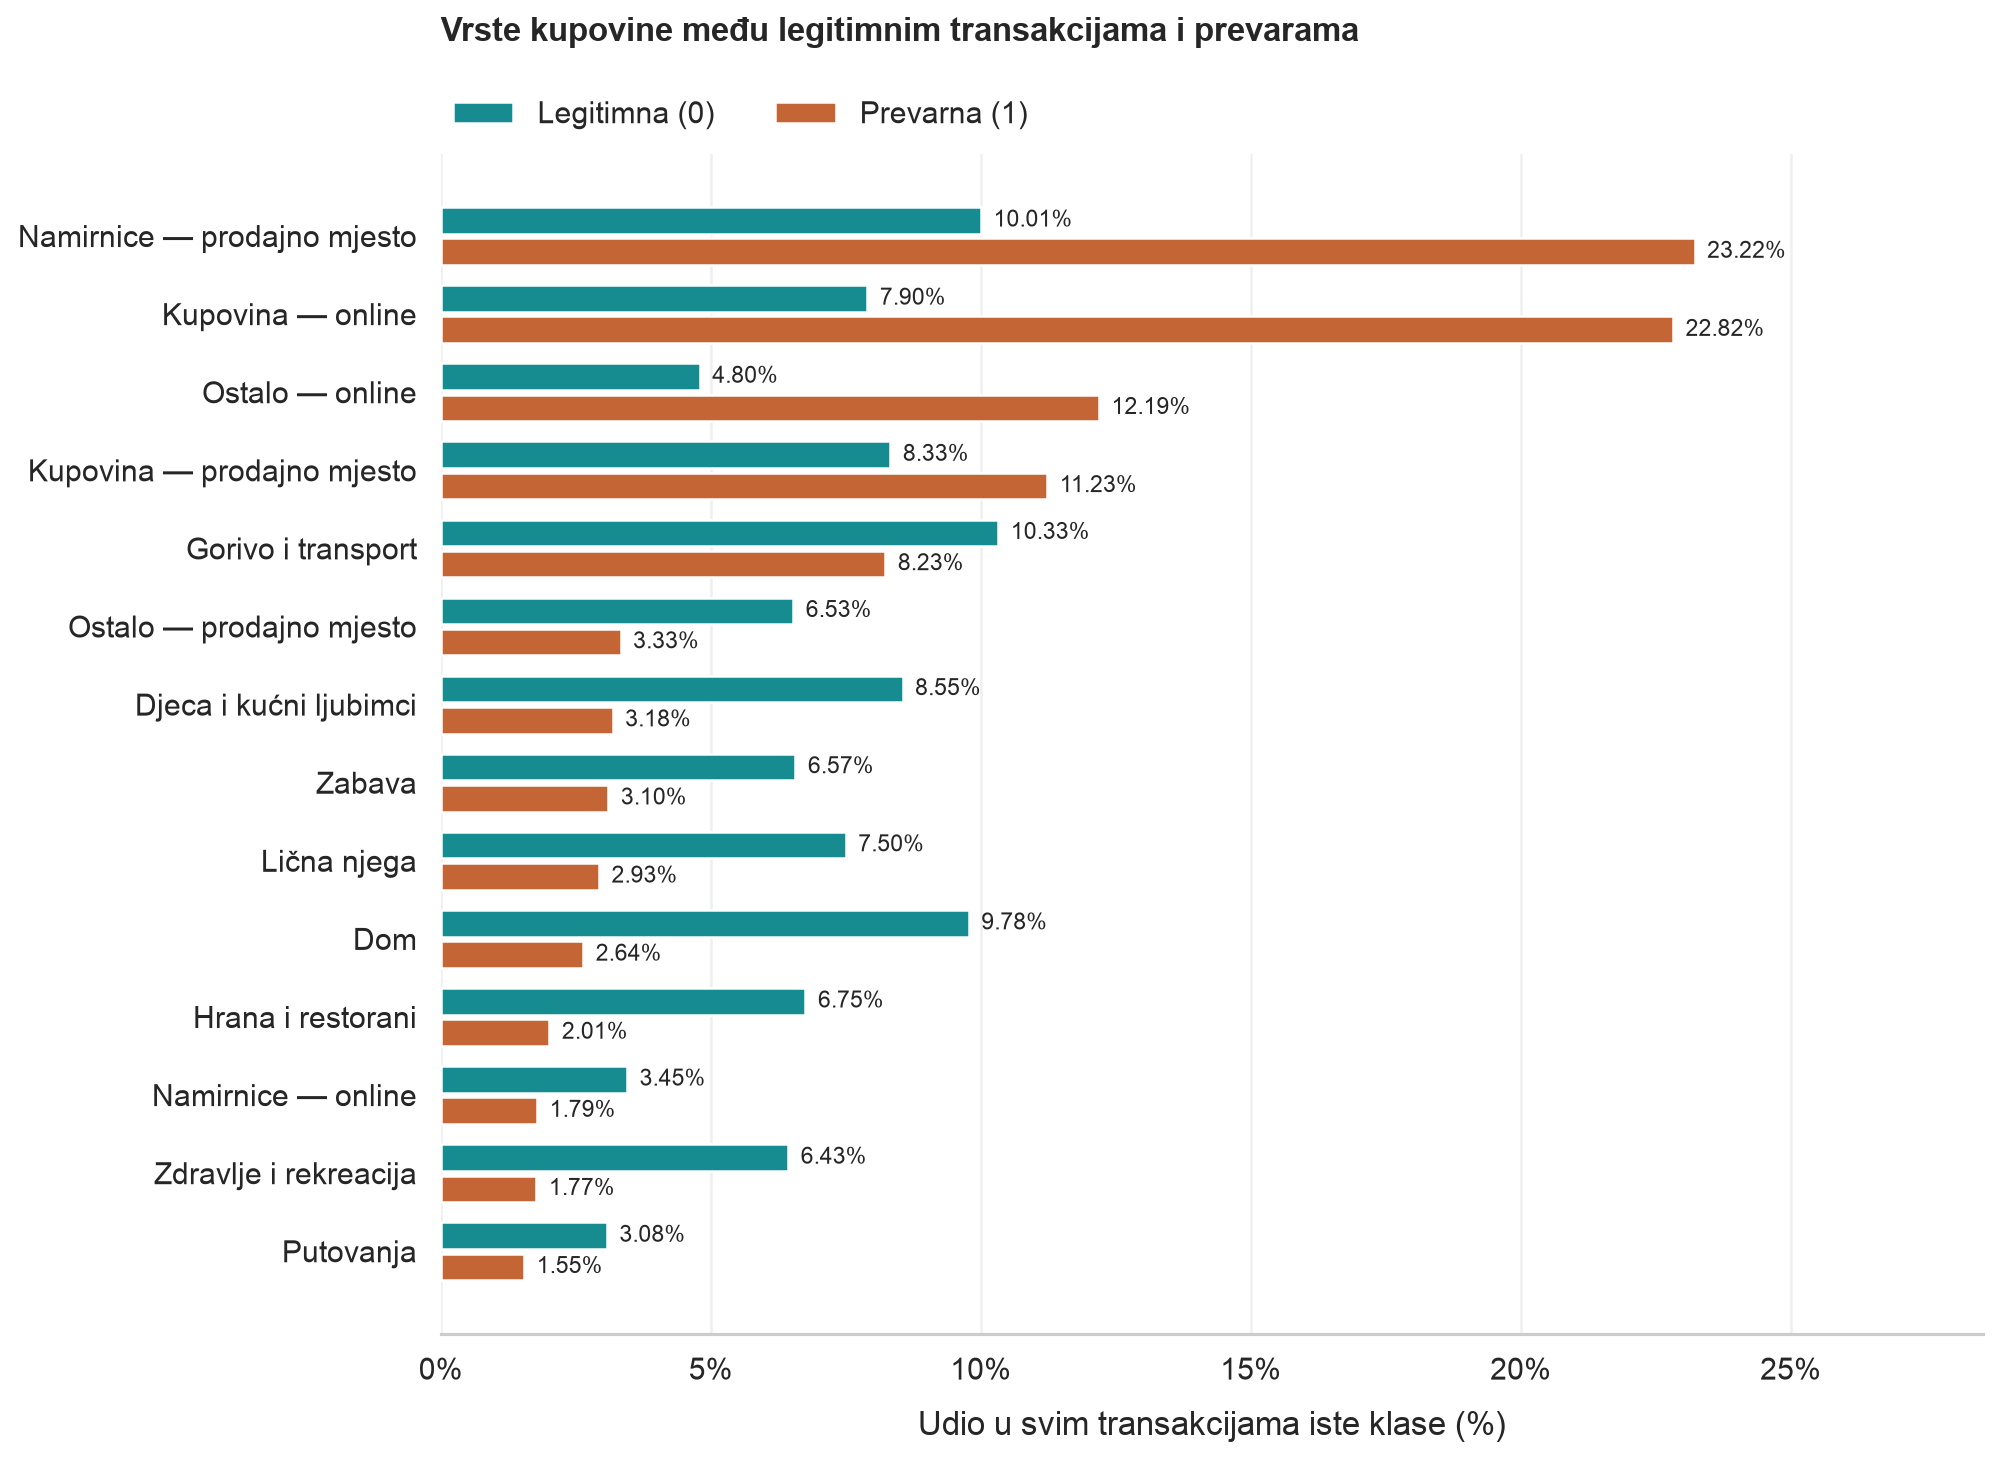
\includegraphics[width=\linewidth,height=.38\textheight,keepaspectratio]{slike/kategorije_po_klasi.png}
\caption{Vrste kupovine po klasi. Svaka klasa zasebno daje zbir 100\,\%, pa se poredi njen unutrašnji sastav.}
\end{figure}


\subsubsection*{Trgovac i zanimanje: veliki broj nominalnih oznaka}
U balansiranom skupu postoji 693 različitih trgovaca i 493 zanimanja. Ove kolone
ne treba tretirati potpuno jednako kao 14 vrsta kupovine. Kod trgovca prosječan
broj zapisa po nazivu je mali, a kod zanimanja se ponavljaju transakcije istih
korisnika. Pojedinačno zanimanje ili trgovac s nekoliko primjera daju ograničenu
osnovu za opis razlika među klasama.

Svi nazivi trgovaca imaju prefiks \texttt{fraud\_}, pa taj dio teksta ne
donosi razliku između klasa. Ostatak naziva predstavlja nominalnu oznaku;
abecedni redoslijed naziva nema mjerno značenje. Prikaz najčešćih trgovaca
pokazuje i da najčešći naziv sam zauzima mali dio ukupnog uzorka.

Zanimanje opisuje korisnika, a ne neposredno svojstvo pojedinačne kupovine.
Jedna osoba zato doprinosi više redova istoj kategoriji zanimanja. Frekvenciju
transakcija ne poistovjećujemo s brojem ljudi zaposlenih u tom zanimanju.
Za rijetke grupe procenat prevara može biti vrlo nestabilan, pa izbor praga
grupisanja zasnivamo na broju zapisa, a ne na njihovom ciljnom ishodu.


\subsubsection*{Grad, savezna država i poštanski broj}
Geografske oznake imaju različitu detaljnost. Savezna država opisuje šire područje,
dok grad i poštanski broj često predstavljaju vrlo specifičnu lokaciju. U
balansiranom skupu ima 889 gradova, 51 savezna država i 964 poštanska broja.
Unija izvora sadrži još više gradova i poštanskih brojeva.

Sam naziv grada ne mora biti jedinstvena lokacija bez konteksta savezne države.
Ni razlika između dva poštanska broja ne predstavlja fizičku udaljenost.
Zato ove oznake nisu uključene u numeričke korelacije. Njihova veza s lokacijom
ispituje se brojem različitih koordinata i kartica po oznaci, uz zadržavanje
činjenice da nazivi i prostorne granice nisu savršeno jednoznačni.
\begin{table}[H]\centering\small
\caption{Geografske oznake i ponovljene lokacije u balansiranom skupu}
\begin{tabularx}{\linewidth}{@{}Yrrr@{}}\toprule
Oznaka & Različitih & Medijan lokacija & Medijan kartica \\ \midrule
city & 889 & 1,00 & 1,00 \\
zip & 964 & 1,00 & 1,00 \\
state & 51 & 17,00 & 17,00 \\
\bottomrule\end{tabularx}\end{table}


\subsubsection*{Spol i šira geografska zastupljenost}
Spol ima dvije kategorije, F i M, bez ordinalnog značenja. Njihove frekvencije
opisuju sastav simuliranih transakcija. One ne predstavljaju broj jedinstvenih
osoba, niti dovoljan osnov za uzročno tumačenje razlika u ishodima.
U pripremi se čuvaju dvije one-hot kolone kako bi prikaz bio neposredno čitljiv.

Savezna država ima 51 nominalnu oznaku u zajedničkom opisu. Za razliku od grada
i poštanskog broja, broj kolona je znatno manji, a oznake pružaju lako tumačiv
regionalni kontekst. Zadržava se cijela raspodjela, uključujući slabije zastupljena
područja. Na malim grupama se ne izvode čvrsti zaključci iz procenta prevara.


\subsubsection*{Identifikatori, imena i adrese}
Broj kartice \texttt{cc\_num} identifikator je koji povezuje više transakcija.
U balansiranom uzorku postoje 977 kartica. Njegova numerička veličina ne opisuje
iznos, redoslijed ponašanja ili udaljenost. Zato računanje prosjeka broja kartice
ili standardizovanje njegovih cifara ne bi imalo korisno mjerno značenje.

Oznaka \texttt{trans\_num} jedinstvena je za svaku transakciju. Njena uloga je
provjera duplikata i preklapanja verzija, te održavanje veze između pripremljenog
reda i izvornog zapisa. Ona se čuva u NPZ metapodacima, a izostavlja iz ulaza.
U kasnijoj podjeli ove oznake omogućavaju provjeru odvojenosti transakcija.

Imena i prezimena nisu jedinstvene oznake osobe. Ista vrijednost može pripadati
različitim korisnicima, dok ponovljene kupovine iste osobe povećavaju frekvenciju
jedne oznake. U balansiranom uzorku najčešće ime je Christopher, a prezime Smith.
Ove frekvencije opisuju sastav uzorka i ne pružaju sadržajno obrazloženje događaja
prevare. Imena i prezimena zato se ne zadržavaju među ulazima.

Adresa \texttt{street} ponavlja se za istog korisnika i izostavlja se s brojem
kartice, imenom i prezimenom. Iz pripreme se uklanjaju samo identifikacijske
kolone; transakcije se ne brišu zbog ponovljenih oznaka.

\begin{figure}[H]\centering
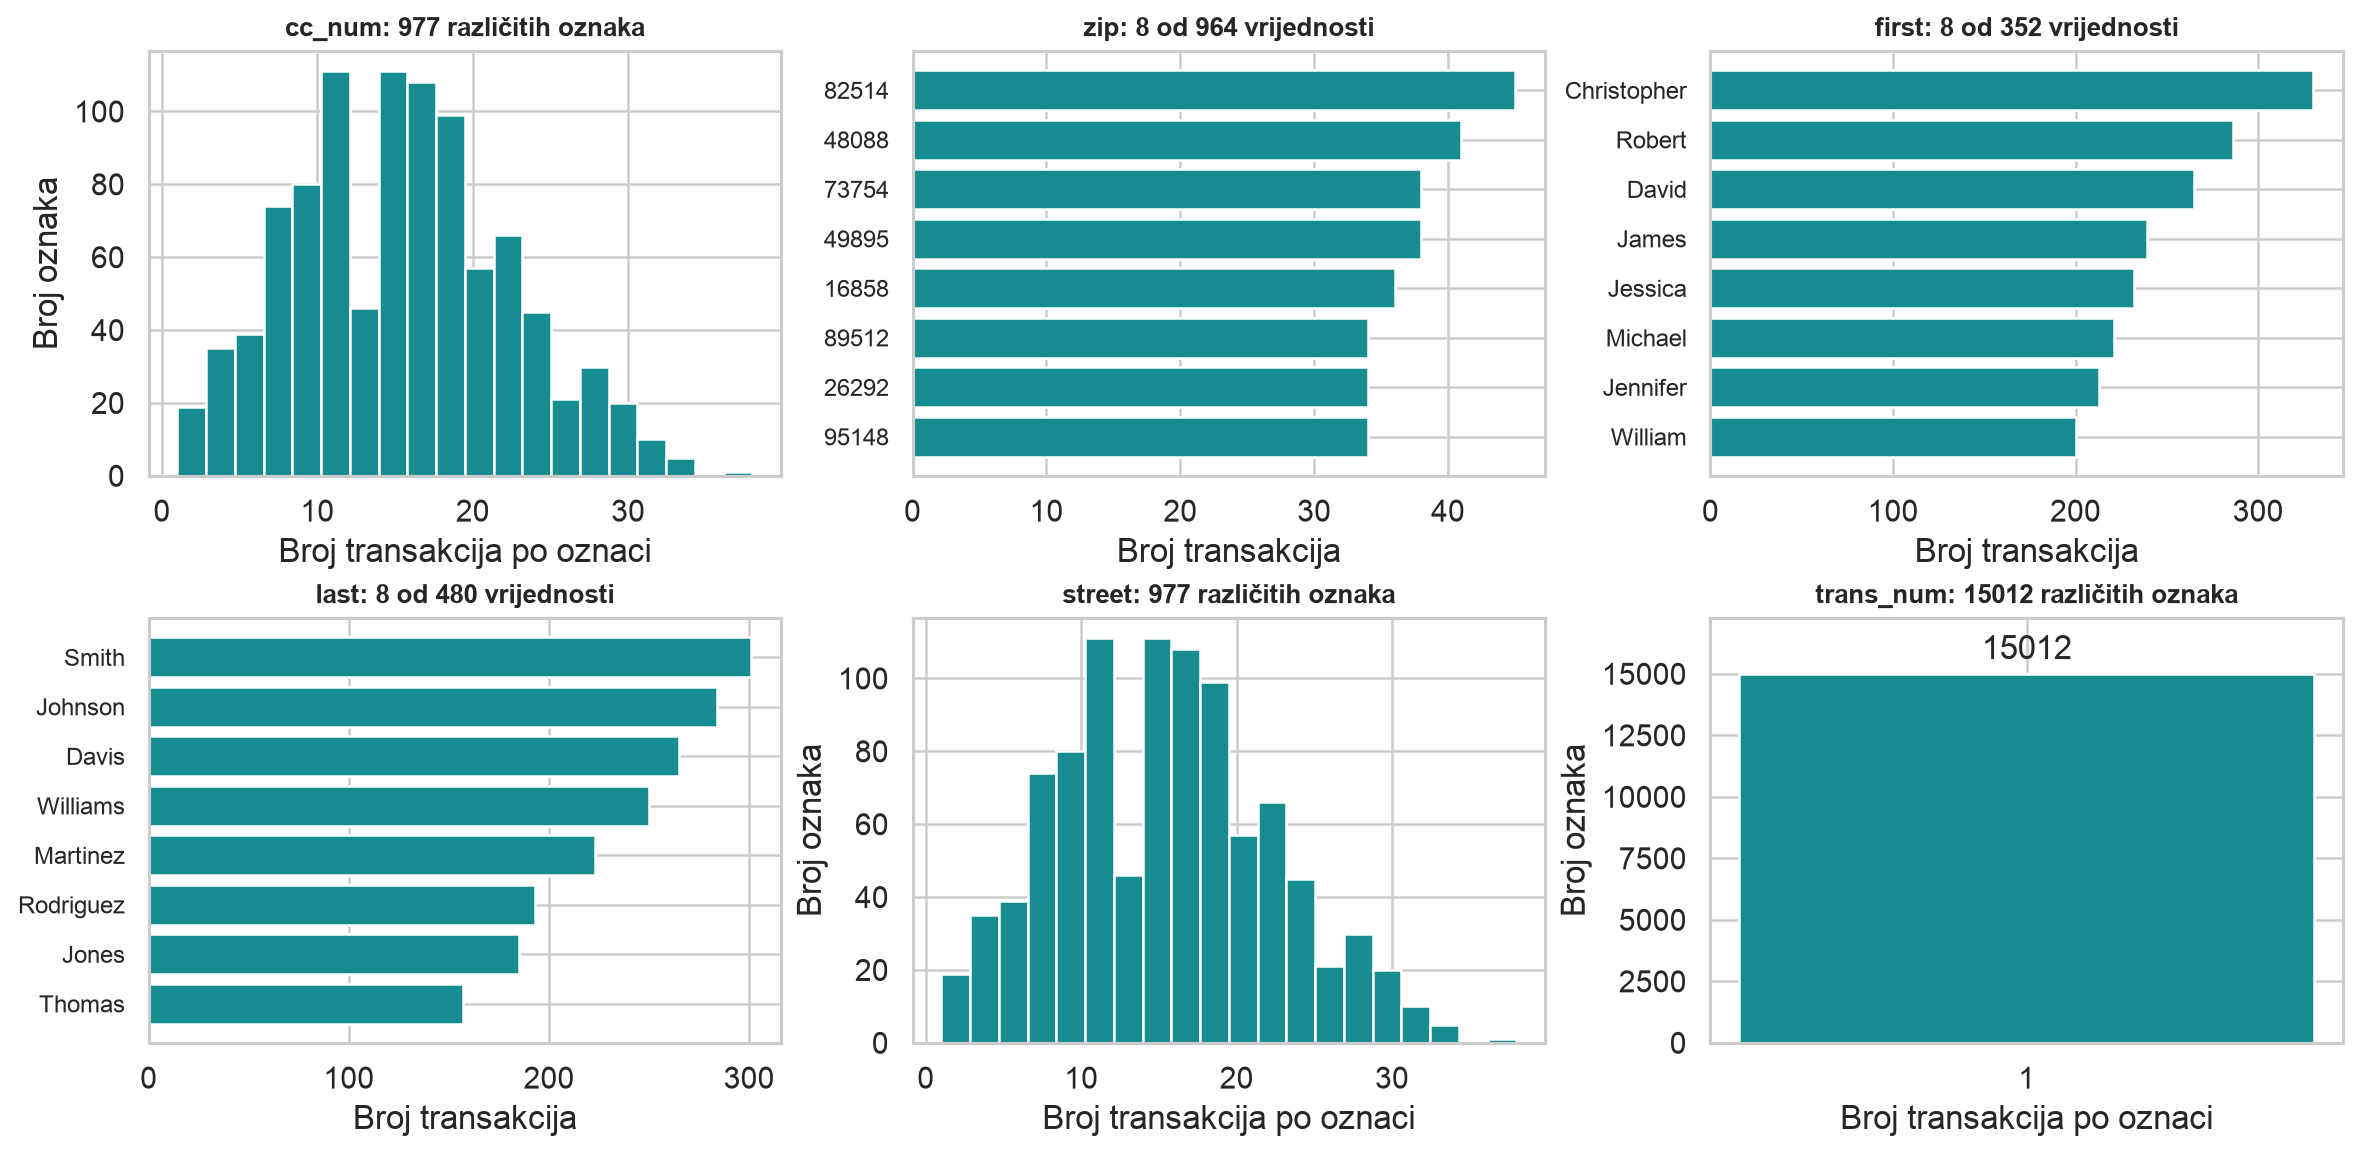
\includegraphics[width=\linewidth,height=.35\textheight,keepaspectratio]{slike/identifikatori.png}
\caption{Ponavljanje kartica i adresa, najčešći poštanski brojevi, imena i prezimena te jedinstvenost oznake transakcije.}
\end{figure}

\subsubsection*{Preklapanje izvora}
Poređenjem \texttt{trans\_num} pronađene su 7\,593 zajedničke transakcije.
Unija dva izvora zato sadrži 22\,419 jedinstvenih transakcija, umjesto zbira
njihovih veličina. Zajednički opisni pretprocesor u 1.4 prilagođava se toj uniji
bez ponovljenih oznaka, kako iste transakcije ne bi dobile dodatnu težinu.

Ponavljanje između dvije verzije je očekivano jer su obje izvedene iz istog
originala. Ono se razlikuje od duplikata unutar jednog CSV-a, kojih nema.
Kod kasnije podjele treba uvažiti zajedničke transakcije tako da izdvojene oznake
za provjeru budu isključene iz odgovarajućih dijelova obje verzije. U ovoj fazi
se ta podjela ne implementira i ne formiraju se dodatni izvozi.


\subsubsection*{Geografski odnosi i izvedena udaljenost}
Raspored koordinata pokazuje koncentracije transakcija na ponovljenim lokacijama.
Na slici su tačke obojene prema klasi samo radi opisa. Preklapanje tačaka i veća
aktivnost pojedinih lokacija otežavaju neposredno poređenje sirovih gustina.
Na osnovu takvog prikaza ne izvodi se zaključak da je određeno područje samo po
sebi uzrok prevare.

Koordinate korisnika i trgovca snažno su povezane, ali male razlike između njih
opisuju prostorni odnos. Haversine udaljenost koristi sve četiri koordinate i
čuva tu razliku u jednoj veličini. Radi se o udaljenosti zračnom linijom na sferi,
a ne dužini putovanja cestom. Zemljin poluprečnik u računu iznosi 6\,371,0088 km.

\begin{figure}[H]\centering
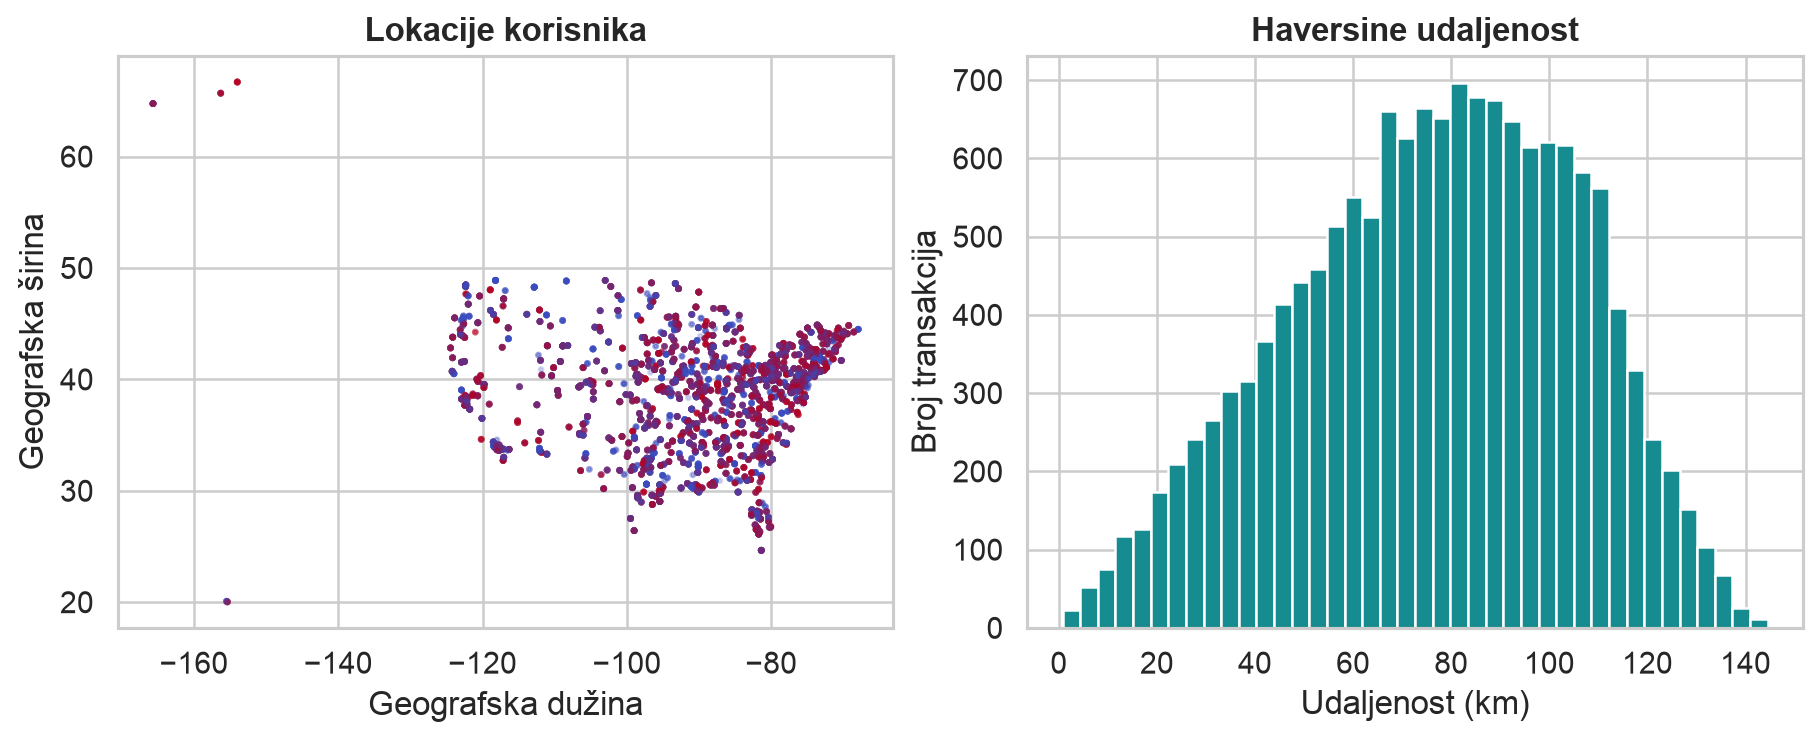
\includegraphics[width=\linewidth,height=.38\textheight,keepaspectratio]{slike/geografski_obrasci.png}
\caption{Raspored lokacija u simuliranom uzorku i raspodjela udaljenosti korisnika od trgovca.}
\end{figure}


\subsubsection*{Pearsonova i Spearmanova povezanost}
Pearsonov koeficijent opisuje linearnu povezanost numeričkih veličina, a
Spearmanov povezanost njihovih rangova. Koristimo oba jer izraženi repovi i
nelinearni odnosi mogu dati različitu sliku. Identifikatori i nominalni kodovi
izostavljeni su iz ovih matrica: njihovo pretvaranje u proizvoljne brojeve
proizvelo bi koeficijente bez opravdanog mjernog značenja.

Povezanost iznosa s ciljem je približno 0,62 po Pearsonu i 0,58 po Spearmanu.
Razlika pokazuje da oba prikaza bilježe odnos u ovom uzorku, ali ne identično.
Slabiji koeficijenti drugih pojedinačnih atributa ne dokazuju da su oni beskorisni:
interakcije i ciklični obrasci nisu potpuno opisani pojedinačnom linearnom vezom.
\begin{table}[H]\centering\small
\caption{Pearsonova i Spearmanova povezanost s ciljem u balansiranom uzorku}
\begin{tabularx}{\linewidth}{@{}Yrr@{}}\toprule
Atribut & Pearson & Spearman \\ \midrule
amt & 0,620 & 0,578 \\
lat & 0,008 & 0,005 \\
long & 0,026 & 0,036 \\
city\_pop & 0,022 & 0,009 \\
unix\_time & -0,032 & -0,032 \\
merch\_lat & 0,008 & 0,004 \\
merch\_long & 0,025 & 0,035 \\
age\_years & 0,068 & 0,063 \\
distance\_km & -0,004 & -0,005 \\
hour & 0,088 & 0,158 \\
day\_of\_week & 0,011 & 0,008 \\
month & -0,078 & -0,087 \\
\bottomrule\end{tabularx}\end{table}

Koeficijenti su opisni za balansirani uzorak i ne potvrđuju uzročnost.

\begin{figure}[H]\centering
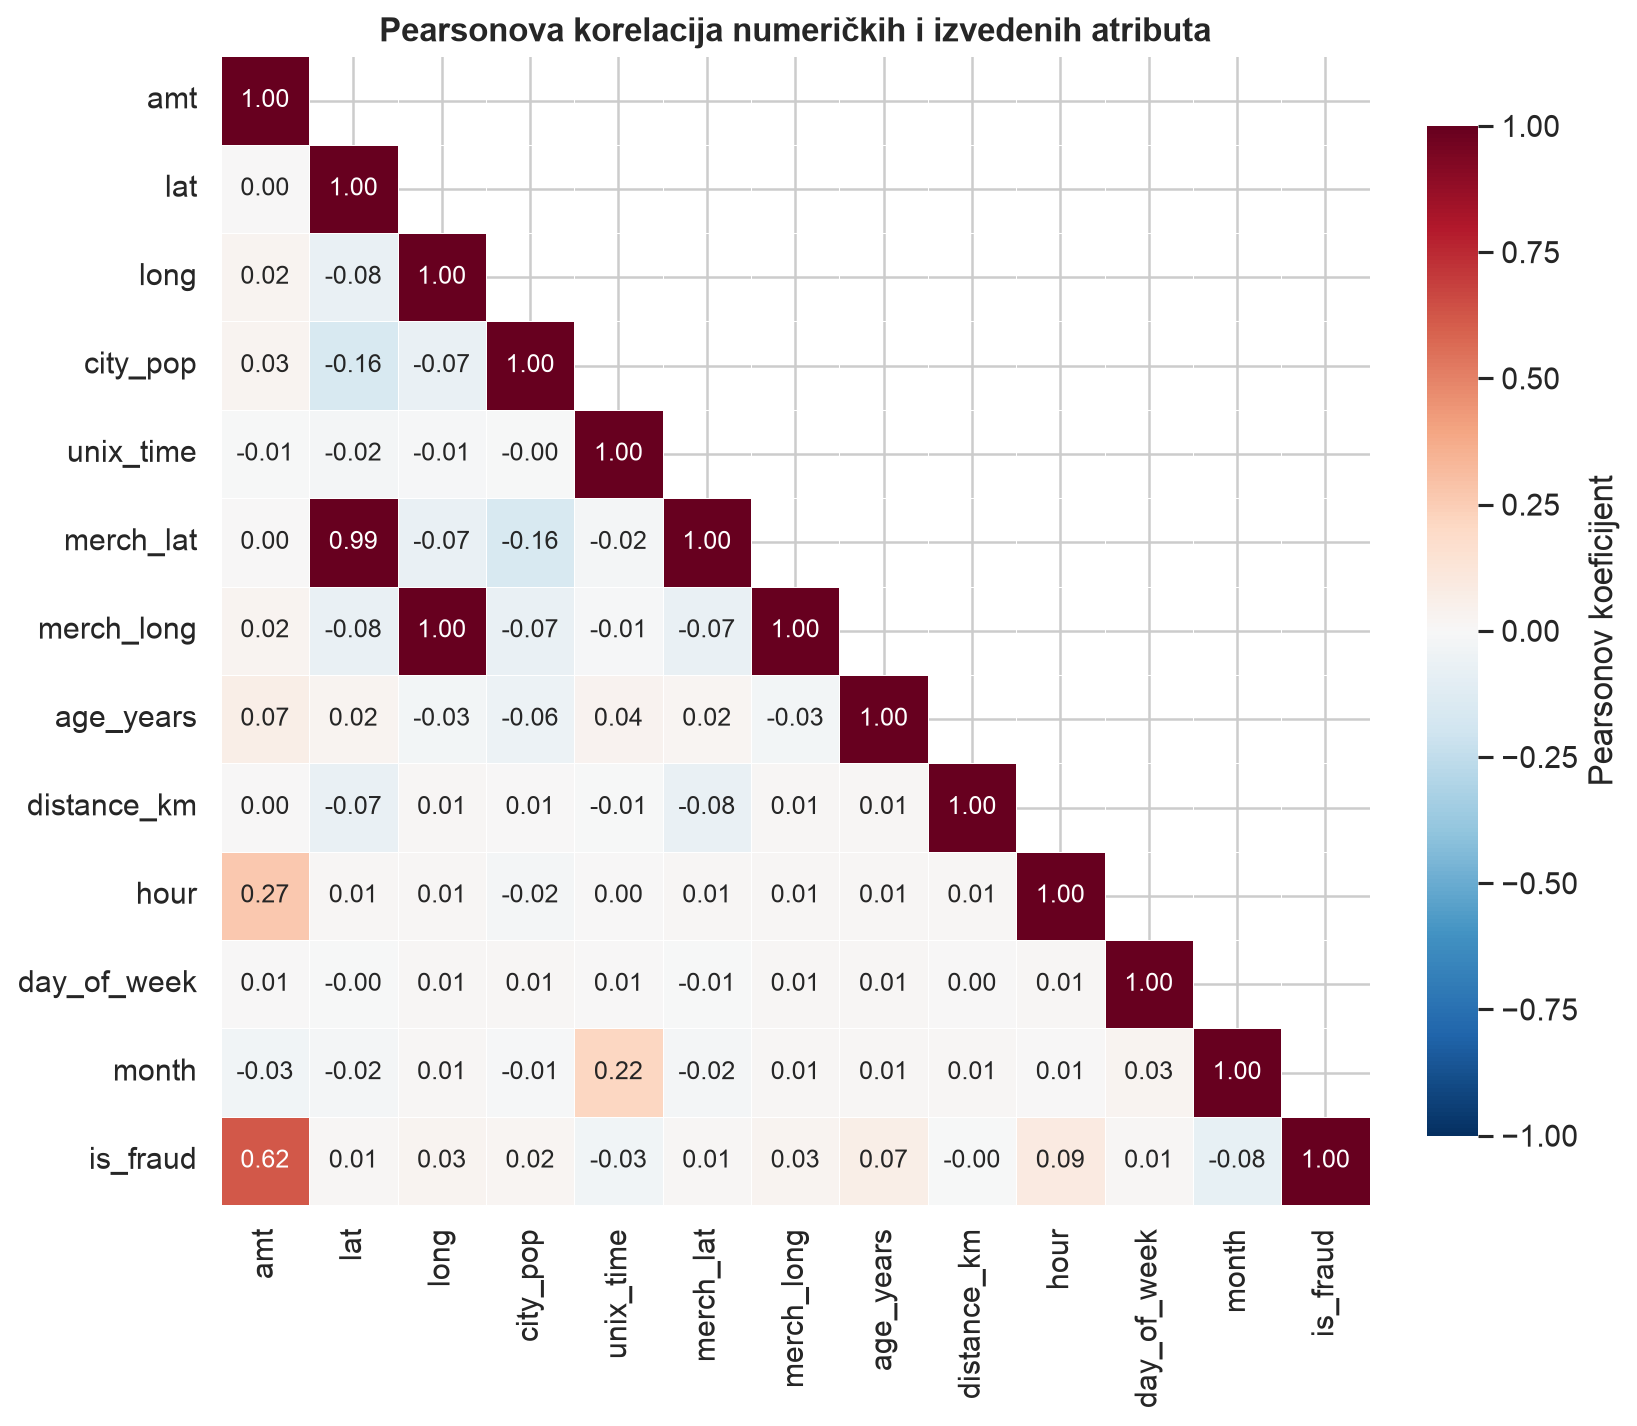
\includegraphics[width=\linewidth,height=.43\textheight,keepaspectratio]{slike/korelacije.png}
\caption{Pearsonova matrica originalnih i izvedenih numeričkih veličina te ciljne klase.}
\end{figure}
